\documentclass{book}
\usepackage[a4paper,top=2.5cm,bottom=2.5cm,left=2.5cm,right=2.5cm]{geometry}
\usepackage{makeidx}
\usepackage{natbib}
\usepackage{graphicx}
\usepackage{multicol}
\usepackage{float}
\usepackage{listings}
\usepackage{color}
\usepackage{ifthen}
\usepackage[table]{xcolor}
\usepackage{textcomp}
\usepackage{alltt}
\usepackage{ifpdf}
\ifpdf
\usepackage[pdftex,
            pagebackref=true,
            colorlinks=true,
            linkcolor=blue,
            unicode
           ]{hyperref}
\else
\usepackage[ps2pdf,
            pagebackref=true,
            colorlinks=true,
            linkcolor=blue,
            unicode
           ]{hyperref}
\usepackage{pspicture}
\fi
\usepackage[utf8]{inputenc}
\usepackage[spanish]{babel}
\usepackage{mathptmx}
\usepackage[scaled=.90]{helvet}
\usepackage{courier}
\usepackage{sectsty}
\usepackage{amssymb}
\usepackage[titles]{tocloft}
\usepackage{doxygen}
\lstset{language=C++,inputencoding=utf8,basicstyle=\footnotesize,breaklines=true,breakatwhitespace=true,tabsize=2,numbers=left }
\makeindex
\setcounter{tocdepth}{3}
\renewcommand{\footrulewidth}{0.4pt}
\renewcommand{\familydefault}{\sfdefault}
\hfuzz=15pt
\setlength{\emergencystretch}{15pt}
\hbadness=750
\tolerance=750
\begin{document}
\hypersetup{pageanchor=false,citecolor=blue}
\begin{titlepage}
\vspace*{7cm}
\begin{center}
{\Large Practica P\-R\-O2. }\\
\vspace*{1cm}
{\large Generado por Doxygen 1.8.2}\\
\vspace*{0.5cm}
{\small Lunes, 9 de Diciembre de 2013 09:11:13}\\
\end{center}
\end{titlepage}
\clearemptydoublepage
\pagenumbering{roman}
\tableofcontents
\clearemptydoublepage
\pagenumbering{arabic}
\hypersetup{pageanchor=true,citecolor=blue}
\chapter{Índice de clases}
\section{Lista de clases}
Lista de las clases, estructuras, uniones e interfaces con una breve descripción\-:\begin{DoxyCompactList}
\item\contentsline{section}{\hyperlink{class_arbre}{Arbre$<$ T $>$} }{\pageref{class_arbre}}{}
\item\contentsline{section}{\hyperlink{class_biblioteca}{Biblioteca} }{\pageref{class_biblioteca}}{}
\item\contentsline{section}{\hyperlink{class_estructura}{Estructura} }{\pageref{class_estructura}}{}
\item\contentsline{section}{\hyperlink{struct_arbre_1_1node__arbre}{Arbre$<$ T $>$\-::node\-\_\-arbre} }{\pageref{struct_arbre_1_1node__arbre}}{}
\item\contentsline{section}{\hyperlink{class_revista}{Revista} }{\pageref{class_revista}}{}
\end{DoxyCompactList}

\chapter{Indice de archivos}
\section{Lista de archivos}
Lista de todos los archivos con descripciones breves\-:\begin{DoxyCompactList}
\item\contentsline{section}{\hyperlink{_arbre_8hpp}{Arbre.\-hpp} }{\pageref{_arbre_8hpp}}{}
\item\contentsline{section}{\hyperlink{biblioteca_8cpp}{biblioteca.\-cpp} }{\pageref{biblioteca_8cpp}}{}
\item\contentsline{section}{\hyperlink{biblioteca_8hpp}{biblioteca.\-hpp} }{\pageref{biblioteca_8hpp}}{}
\item\contentsline{section}{\hyperlink{estructura_8cpp}{estructura.\-cpp} }{\pageref{estructura_8cpp}}{}
\item\contentsline{section}{\hyperlink{estructura_8hpp}{estructura.\-hpp} }{\pageref{estructura_8hpp}}{}
\item\contentsline{section}{\hyperlink{pro2_8cpp}{pro2.\-cpp} }{\pageref{pro2_8cpp}}{}
\item\contentsline{section}{\hyperlink{revista_8cpp}{revista.\-cpp} }{\pageref{revista_8cpp}}{}
\item\contentsline{section}{\hyperlink{revista_8hpp}{revista.\-hpp} }{\pageref{revista_8hpp}}{}
\end{DoxyCompactList}

\chapter{Documentación de las clases}
\hypertarget{class_arbre}{\section{Referencia de la plantilla de la Clase Arbre$<$ T $>$}
\label{class_arbre}\index{Arbre$<$ T $>$@{Arbre$<$ T $>$}}
}
\subsection*{Clases}
\begin{DoxyCompactItemize}
\item 
struct \hyperlink{struct_arbre_1_1node__arbre}{node\-\_\-arbre}
\end{DoxyCompactItemize}
\subsection*{Métodos públicos}
\begin{DoxyCompactItemize}
\item 
\hyperlink{class_arbre_a3f613426983169266297eb841996845e}{Arbre} ()
\item 
\hyperlink{class_arbre_a8f8615c19988334f9b77dc51f44acc6d}{Arbre} (const \hyperlink{class_arbre}{Arbre} \&original)
\item 
\hyperlink{class_arbre_a13cfb8184d9c43d92584d434243c7b3d}{$\sim$\-Arbre} ()
\item 
\hyperlink{class_arbre}{Arbre} \& \hyperlink{class_arbre_a58314b830f6f3ba0e598e352513a87c5}{operator=} (const \hyperlink{class_arbre}{Arbre} \&original)
\item 
void \hyperlink{class_arbre_aa74ec0d2b601487b822eb70100330582}{a\-\_\-buit} ()
\item 
void \hyperlink{class_arbre_a931d1c91e9fd6cbe72703a7ba7d40415}{swap} (\hyperlink{class_arbre}{Arbre} \&a)
\item 
void \hyperlink{class_arbre_a806d45f6f1d3a9dd357563979186f721}{plantar} (const T \&x, \hyperlink{class_arbre}{Arbre} \&a1, \hyperlink{class_arbre}{Arbre} \&a2)
\item 
void \hyperlink{class_arbre_aee75355cee7599e132de75781d26a61d}{fills} (\hyperlink{class_arbre}{Arbre} \&fe, \hyperlink{class_arbre}{Arbre} \&fd)
\item 
T \hyperlink{class_arbre_aa6e2559ead7dfceda962cff11fb1a15c}{arrel} () const 
\item 
bool \hyperlink{class_arbre_a68a51f6689f0b2889e8e1d56266fd620}{es\-\_\-buit} () const 
\end{DoxyCompactItemize}
\subsection*{Métodos privados}
\begin{DoxyCompactItemize}
\item 
\hyperlink{struct_arbre_1_1node__arbre}{node\-\_\-arbre} $\ast$ \hyperlink{class_arbre_a8562c3574c0037eae30a6d04050fb517}{copia\-\_\-node\-\_\-arbre} (\hyperlink{struct_arbre_1_1node__arbre}{node\-\_\-arbre} $\ast$m)
\item 
void \hyperlink{class_arbre_ab97c98d266a5b8973fe2519c14cf362a}{esborra\-\_\-node\-\_\-arbre} (\hyperlink{struct_arbre_1_1node__arbre}{node\-\_\-arbre} $\ast$m)
\end{DoxyCompactItemize}
\subsection*{Atributos privados}
\begin{DoxyCompactItemize}
\item 
\hyperlink{struct_arbre_1_1node__arbre}{node\-\_\-arbre} $\ast$ \hyperlink{class_arbre_a62818cdde6c1912a7c9a15db3b93d297}{primer\-\_\-node}
\end{DoxyCompactItemize}


\subsection{Descripción detallada}
\subsubsection*{template$<$class T$>$class Arbre$<$ T $>$}



Definición en la línea 6 del archivo Arbre.\-hpp.



\subsection{Documentación del constructor y destructor}
\hypertarget{class_arbre_a3f613426983169266297eb841996845e}{\index{Arbre@{Arbre}!Arbre@{Arbre}}
\index{Arbre@{Arbre}!Arbre@{Arbre}}
\subsubsection[{Arbre}]{\setlength{\rightskip}{0pt plus 5cm}template$<$class T$>$ {\bf Arbre}$<$ T $>$\-::{\bf Arbre} (
\begin{DoxyParamCaption}
{}
\end{DoxyParamCaption}
)}}\label{class_arbre_a3f613426983169266297eb841996845e}


Definición en la línea 55 del archivo Arbre.\-hpp.


\begin{DoxyCode}
  \{
    \hyperlink{class_arbre_a62818cdde6c1912a7c9a15db3b93d297}{primer\_node}= NULL;
  \}
\end{DoxyCode}
\hypertarget{class_arbre_a8f8615c19988334f9b77dc51f44acc6d}{\index{Arbre@{Arbre}!Arbre@{Arbre}}
\index{Arbre@{Arbre}!Arbre@{Arbre}}
\subsubsection[{Arbre}]{\setlength{\rightskip}{0pt plus 5cm}template$<$class T$>$ {\bf Arbre}$<$ T $>$\-::{\bf Arbre} (
\begin{DoxyParamCaption}
\item[{const {\bf Arbre}$<$ T $>$ \&}]{original}
\end{DoxyParamCaption}
)}}\label{class_arbre_a8f8615c19988334f9b77dc51f44acc6d}


Definición en la línea 62 del archivo Arbre.\-hpp.


\begin{DoxyCode}
  \{
    \textcolor{keywordflow}{if} (\textcolor{keyword}{this} != &original)     
      \hyperlink{class_arbre_a62818cdde6c1912a7c9a15db3b93d297}{primer\_node} = \hyperlink{class_arbre_a8562c3574c0037eae30a6d04050fb517}{copia\_node\_arbre}(original.
      \hyperlink{class_arbre_a62818cdde6c1912a7c9a15db3b93d297}{primer\_node});
  \}
\end{DoxyCode}
\hypertarget{class_arbre_a13cfb8184d9c43d92584d434243c7b3d}{\index{Arbre@{Arbre}!$\sim$\-Arbre@{$\sim$\-Arbre}}
\index{$\sim$\-Arbre@{$\sim$\-Arbre}!Arbre@{Arbre}}
\subsubsection[{$\sim$\-Arbre}]{\setlength{\rightskip}{0pt plus 5cm}template$<$class T$>$ {\bf Arbre}$<$ T $>$\-::$\sim${\bf Arbre} (
\begin{DoxyParamCaption}
{}
\end{DoxyParamCaption}
)}}\label{class_arbre_a13cfb8184d9c43d92584d434243c7b3d}


Definición en la línea 70 del archivo Arbre.\-hpp.


\begin{DoxyCode}
           \{
    \hyperlink{class_arbre_ab97c98d266a5b8973fe2519c14cf362a}{esborra\_node\_arbre}(\hyperlink{class_arbre_a62818cdde6c1912a7c9a15db3b93d297}{primer\_node});
  \}
\end{DoxyCode}


\subsection{Documentación de las funciones miembro}
\hypertarget{class_arbre_a8562c3574c0037eae30a6d04050fb517}{\index{Arbre@{Arbre}!copia\-\_\-node\-\_\-arbre@{copia\-\_\-node\-\_\-arbre}}
\index{copia\-\_\-node\-\_\-arbre@{copia\-\_\-node\-\_\-arbre}!Arbre@{Arbre}}
\subsubsection[{copia\-\_\-node\-\_\-arbre}]{\setlength{\rightskip}{0pt plus 5cm}template$<$class T$>$ {\bf node\-\_\-arbre}$\ast$ {\bf Arbre}$<$ T $>$\-::copia\-\_\-node\-\_\-arbre (
\begin{DoxyParamCaption}
\item[{{\bf node\-\_\-arbre} $\ast$}]{m}
\end{DoxyParamCaption}
)\hspace{0.3cm}{\ttfamily [private]}}}\label{class_arbre_a8562c3574c0037eae30a6d04050fb517}


Definición en la línea 20 del archivo Arbre.\-hpp.


\begin{DoxyCode}
  \{
    node\_arbre* n;
    \textcolor{keywordflow}{if} (m==NULL) n=NULL;
    \textcolor{keywordflow}{else} \{
      n = \textcolor{keyword}{new} node\_arbre;
      n->info = m->info;
      n->segE = \hyperlink{class_arbre_a8562c3574c0037eae30a6d04050fb517}{copia\_node\_arbre}(m->segE);
      n->segD = \hyperlink{class_arbre_a8562c3574c0037eae30a6d04050fb517}{copia\_node\_arbre}(m->segD);
    \}
    \textcolor{keywordflow}{return} n;
  \}
\end{DoxyCode}
\hypertarget{class_arbre_ab97c98d266a5b8973fe2519c14cf362a}{\index{Arbre@{Arbre}!esborra\-\_\-node\-\_\-arbre@{esborra\-\_\-node\-\_\-arbre}}
\index{esborra\-\_\-node\-\_\-arbre@{esborra\-\_\-node\-\_\-arbre}!Arbre@{Arbre}}
\subsubsection[{esborra\-\_\-node\-\_\-arbre}]{\setlength{\rightskip}{0pt plus 5cm}template$<$class T$>$ void {\bf Arbre}$<$ T $>$\-::esborra\-\_\-node\-\_\-arbre (
\begin{DoxyParamCaption}
\item[{{\bf node\-\_\-arbre} $\ast$}]{m}
\end{DoxyParamCaption}
)\hspace{0.3cm}{\ttfamily [private]}}}\label{class_arbre_ab97c98d266a5b8973fe2519c14cf362a}


Definición en la línea 38 del archivo Arbre.\-hpp.


\begin{DoxyCode}
  \{
    \textcolor{keywordflow}{if} (m != NULL) \{
      \hyperlink{class_arbre_ab97c98d266a5b8973fe2519c14cf362a}{esborra\_node\_arbre}(m->segE);
      \hyperlink{class_arbre_ab97c98d266a5b8973fe2519c14cf362a}{esborra\_node\_arbre}(m->segD);
      \textcolor{keyword}{delete} m;
    \}
  \}
\end{DoxyCode}
\hypertarget{class_arbre_a58314b830f6f3ba0e598e352513a87c5}{\index{Arbre@{Arbre}!operator=@{operator=}}
\index{operator=@{operator=}!Arbre@{Arbre}}
\subsubsection[{operator=}]{\setlength{\rightskip}{0pt plus 5cm}template$<$class T$>$ {\bf Arbre}\& {\bf Arbre}$<$ T $>$\-::operator= (
\begin{DoxyParamCaption}
\item[{const {\bf Arbre}$<$ T $>$ \&}]{original}
\end{DoxyParamCaption}
)}}\label{class_arbre_a58314b830f6f3ba0e598e352513a87c5}


Definición en la línea 74 del archivo Arbre.\-hpp.


\begin{DoxyCode}
                                          \{
    \textcolor{keywordflow}{if} (\textcolor{keyword}{this} != &original) \{
      \hyperlink{class_arbre_ab97c98d266a5b8973fe2519c14cf362a}{esborra\_node\_arbre}(\hyperlink{class_arbre_a62818cdde6c1912a7c9a15db3b93d297}{primer\_node});
      \hyperlink{class_arbre_a62818cdde6c1912a7c9a15db3b93d297}{primer\_node} = \hyperlink{class_arbre_a8562c3574c0037eae30a6d04050fb517}{copia\_node\_arbre}(original.
      \hyperlink{class_arbre_a62818cdde6c1912a7c9a15db3b93d297}{primer\_node});
    \}
    \textcolor{keywordflow}{return} *\textcolor{keyword}{this};
  \}
\end{DoxyCode}
\hypertarget{class_arbre_aa74ec0d2b601487b822eb70100330582}{\index{Arbre@{Arbre}!a\-\_\-buit@{a\-\_\-buit}}
\index{a\-\_\-buit@{a\-\_\-buit}!Arbre@{Arbre}}
\subsubsection[{a\-\_\-buit}]{\setlength{\rightskip}{0pt plus 5cm}template$<$class T$>$ void {\bf Arbre}$<$ T $>$\-::a\-\_\-buit (
\begin{DoxyParamCaption}
{}
\end{DoxyParamCaption}
)}}\label{class_arbre_aa74ec0d2b601487b822eb70100330582}


Definición en la línea 82 del archivo Arbre.\-hpp.


\begin{DoxyCode}
  \{
    \hyperlink{class_arbre_ab97c98d266a5b8973fe2519c14cf362a}{esborra\_node\_arbre}(\hyperlink{class_arbre_a62818cdde6c1912a7c9a15db3b93d297}{primer\_node});
    \hyperlink{class_arbre_a62818cdde6c1912a7c9a15db3b93d297}{primer\_node}= NULL;
  \}  
\end{DoxyCode}
\hypertarget{class_arbre_a931d1c91e9fd6cbe72703a7ba7d40415}{\index{Arbre@{Arbre}!swap@{swap}}
\index{swap@{swap}!Arbre@{Arbre}}
\subsubsection[{swap}]{\setlength{\rightskip}{0pt plus 5cm}template$<$class T$>$ void {\bf Arbre}$<$ T $>$\-::swap (
\begin{DoxyParamCaption}
\item[{{\bf Arbre}$<$ T $>$ \&}]{a}
\end{DoxyParamCaption}
)}}\label{class_arbre_a931d1c91e9fd6cbe72703a7ba7d40415}


Definición en la línea 90 del archivo Arbre.\-hpp.


\begin{DoxyCode}
  \{
    node\_arbre* aux;
    aux = a.\hyperlink{class_arbre_a62818cdde6c1912a7c9a15db3b93d297}{primer\_node};
    a.\hyperlink{class_arbre_a62818cdde6c1912a7c9a15db3b93d297}{primer\_node} = \hyperlink{class_arbre_a62818cdde6c1912a7c9a15db3b93d297}{primer\_node};
    \hyperlink{class_arbre_a62818cdde6c1912a7c9a15db3b93d297}{primer\_node} = aux;
  \}
\end{DoxyCode}
\hypertarget{class_arbre_a806d45f6f1d3a9dd357563979186f721}{\index{Arbre@{Arbre}!plantar@{plantar}}
\index{plantar@{plantar}!Arbre@{Arbre}}
\subsubsection[{plantar}]{\setlength{\rightskip}{0pt plus 5cm}template$<$class T$>$ void {\bf Arbre}$<$ T $>$\-::plantar (
\begin{DoxyParamCaption}
\item[{const T \&}]{x, }
\item[{{\bf Arbre}$<$ T $>$ \&}]{a1, }
\item[{{\bf Arbre}$<$ T $>$ \&}]{a2}
\end{DoxyParamCaption}
)}}\label{class_arbre_a806d45f6f1d3a9dd357563979186f721}


Definición en la línea 100 del archivo Arbre.\-hpp.


\begin{DoxyCode}
  \{
    \textcolor{keywordflow}{if} (\textcolor{keyword}{this} != &a1 and \textcolor{keyword}{this} != &a2) \{
      \textcolor{keywordflow}{if} (\hyperlink{class_arbre_a62818cdde6c1912a7c9a15db3b93d297}{primer\_node}==NULL) \{
        node\_arbre* aux;
        aux= \textcolor{keyword}{new} node\_arbre;
        aux->info= x;
        aux->segE= a1.\hyperlink{class_arbre_a62818cdde6c1912a7c9a15db3b93d297}{primer\_node};
        \textcolor{keywordflow}{if} (a1.\hyperlink{class_arbre_a62818cdde6c1912a7c9a15db3b93d297}{primer\_node} == a2.\hyperlink{class_arbre_a62818cdde6c1912a7c9a15db3b93d297}{primer\_node}) aux->\hyperlink{struct_arbre_1_1node__arbre_a9986e206810ba9e519b5b6e590238093}{segD}
      = \hyperlink{class_arbre_a8562c3574c0037eae30a6d04050fb517}{copia\_node\_arbre}(a1.\hyperlink{class_arbre_a62818cdde6c1912a7c9a15db3b93d297}{primer\_node});
        \textcolor{keywordflow}{else}  aux->segD= a2.\hyperlink{class_arbre_a62818cdde6c1912a7c9a15db3b93d297}{primer\_node};
        \hyperlink{class_arbre_a62818cdde6c1912a7c9a15db3b93d297}{primer\_node}= aux;
        a1.\hyperlink{class_arbre_a62818cdde6c1912a7c9a15db3b93d297}{primer\_node}= NULL;
        a2.\hyperlink{class_arbre_a62818cdde6c1912a7c9a15db3b93d297}{primer\_node}= NULL;
      \}
      \textcolor{keywordflow}{else}
        \textcolor{keywordflow}{throw} PRO2Excepcio (\textcolor{stringliteral}{"El p.i. de plantar ha de ser buit a la crida"});
    \}
    \textcolor{keywordflow}{else}
      \textcolor{keywordflow}{throw} PRO2Excepcio (\textcolor{stringliteral}{"El p.i. de plantar no pot coincidir amb els par�metres
      "});    
  \}
\end{DoxyCode}
\hypertarget{class_arbre_aee75355cee7599e132de75781d26a61d}{\index{Arbre@{Arbre}!fills@{fills}}
\index{fills@{fills}!Arbre@{Arbre}}
\subsubsection[{fills}]{\setlength{\rightskip}{0pt plus 5cm}template$<$class T$>$ void {\bf Arbre}$<$ T $>$\-::fills (
\begin{DoxyParamCaption}
\item[{{\bf Arbre}$<$ T $>$ \&}]{fe, }
\item[{{\bf Arbre}$<$ T $>$ \&}]{fd}
\end{DoxyParamCaption}
)}}\label{class_arbre_aee75355cee7599e132de75781d26a61d}


Definición en la línea 126 del archivo Arbre.\-hpp.


\begin{DoxyCode}
  \{
    \textcolor{keywordflow}{if} (\hyperlink{class_arbre_a62818cdde6c1912a7c9a15db3b93d297}{primer\_node}!=NULL and fe.\hyperlink{class_arbre_a62818cdde6c1912a7c9a15db3b93d297}{primer\_node}==NULL
        and fd.\hyperlink{class_arbre_a62818cdde6c1912a7c9a15db3b93d297}{primer\_node}==NULL) \{
      \textcolor{keywordflow}{if} (&fe != &fd) \{       
        node\_arbre* aux;
        aux= \hyperlink{class_arbre_a62818cdde6c1912a7c9a15db3b93d297}{primer\_node};
        fe.\hyperlink{class_arbre_a62818cdde6c1912a7c9a15db3b93d297}{primer\_node}= aux->\hyperlink{struct_arbre_1_1node__arbre_add2e7f2ee789db9f38a3bf2d2dd36972}{segE};
        fd.\hyperlink{class_arbre_a62818cdde6c1912a7c9a15db3b93d297}{primer\_node}= aux->\hyperlink{struct_arbre_1_1node__arbre_a9986e206810ba9e519b5b6e590238093}{segD};
        \hyperlink{class_arbre_a62818cdde6c1912a7c9a15db3b93d297}{primer\_node}= NULL;
        \textcolor{keyword}{delete} aux;
      \}
      \textcolor{keywordflow}{else} 
        \textcolor{keywordflow}{throw} PRO2Excepcio 
              (\textcolor{stringliteral}{"Els dos par�metres de fills no poden coincidir"});      
    \}
    \textcolor{keywordflow}{else} \textcolor{keywordflow}{if} (\hyperlink{class_arbre_a62818cdde6c1912a7c9a15db3b93d297}{primer\_node}==NULL)
      \textcolor{keywordflow}{throw} PRO2Excepcio (\textcolor{stringliteral}{"Un arbre buit no t� fills"});
    \textcolor{keywordflow}{else}   
      \textcolor{keywordflow}{throw} PRO2Excepcio 
        (\textcolor{stringliteral}{"Els dos par�metres de fills han de ser buits a la crida"});  
  \}
\end{DoxyCode}
\hypertarget{class_arbre_aa6e2559ead7dfceda962cff11fb1a15c}{\index{Arbre@{Arbre}!arrel@{arrel}}
\index{arrel@{arrel}!Arbre@{Arbre}}
\subsubsection[{arrel}]{\setlength{\rightskip}{0pt plus 5cm}template$<$class T$>$ T {\bf Arbre}$<$ T $>$\-::arrel (
\begin{DoxyParamCaption}
{}
\end{DoxyParamCaption}
) const}}\label{class_arbre_aa6e2559ead7dfceda962cff11fb1a15c}


Definición en la línea 152 del archivo Arbre.\-hpp.


\begin{DoxyCode}
  \{
    \textcolor{keywordflow}{if} (\hyperlink{class_arbre_a62818cdde6c1912a7c9a15db3b93d297}{primer\_node}!=NULL)
      \textcolor{keywordflow}{return} \hyperlink{class_arbre_a62818cdde6c1912a7c9a15db3b93d297}{primer\_node}->\hyperlink{struct_arbre_1_1node__arbre_a5a146e5e27a7a6c5f54bc6df864595aa}{info};    
    \textcolor{keywordflow}{else}
      \textcolor{keywordflow}{throw} PRO2Excepcio (\textcolor{stringliteral}{"Un arbre buit no t� arrel"});
  \}
\end{DoxyCode}
\hypertarget{class_arbre_a68a51f6689f0b2889e8e1d56266fd620}{\index{Arbre@{Arbre}!es\-\_\-buit@{es\-\_\-buit}}
\index{es\-\_\-buit@{es\-\_\-buit}!Arbre@{Arbre}}
\subsubsection[{es\-\_\-buit}]{\setlength{\rightskip}{0pt plus 5cm}template$<$class T$>$ bool {\bf Arbre}$<$ T $>$\-::es\-\_\-buit (
\begin{DoxyParamCaption}
{}
\end{DoxyParamCaption}
) const}}\label{class_arbre_a68a51f6689f0b2889e8e1d56266fd620}


Definición en la línea 162 del archivo Arbre.\-hpp.


\begin{DoxyCode}
  \{
    \textcolor{keywordflow}{return} (\hyperlink{class_arbre_a62818cdde6c1912a7c9a15db3b93d297}{primer\_node}==NULL);
  \}
\end{DoxyCode}


\subsection{Documentación de los datos miembro}
\hypertarget{class_arbre_a62818cdde6c1912a7c9a15db3b93d297}{\index{Arbre@{Arbre}!primer\-\_\-node@{primer\-\_\-node}}
\index{primer\-\_\-node@{primer\-\_\-node}!Arbre@{Arbre}}
\subsubsection[{primer\-\_\-node}]{\setlength{\rightskip}{0pt plus 5cm}template$<$class T$>$ {\bf node\-\_\-arbre}$\ast$ {\bf Arbre}$<$ T $>$\-::primer\-\_\-node\hspace{0.3cm}{\ttfamily [private]}}}\label{class_arbre_a62818cdde6c1912a7c9a15db3b93d297}


Definición en la línea 16 del archivo Arbre.\-hpp.



La documentación para esta clase fue generada a partir del siguiente fichero\-:\begin{DoxyCompactItemize}
\item 
\hyperlink{_arbre_8hpp}{Arbre.\-hpp}\end{DoxyCompactItemize}

\hypertarget{class_biblioteca}{\section{Referencia de la Clase Biblioteca}
\label{class_biblioteca}\index{Biblioteca@{Biblioteca}}
}
\subsection*{Métodos públicos}
\begin{DoxyCompactItemize}
\item 
void \hyperlink{class_biblioteca_ac95f8ebef5693712c51ab157632b4a27}{anadir\-\_\-revista} (\hyperlink{class_revista}{Revista} \&r)
\begin{DoxyCompactList}\small\item\em Añadir revista. \end{DoxyCompactList}\item 
\hyperlink{class_biblioteca_a442743666a699393ac7ec7ee5d5a33ee}{Biblioteca} (int n)
\item 
void \hyperlink{class_biblioteca_a903cc3f25beff06e4d59b90968890d4f}{eliminar\-\_\-revista} (const string nombre)
\begin{DoxyCompactList}\small\item\em Eliminar revista. \end{DoxyCompactList}\item 
void \hyperlink{class_biblioteca_a44ee151b8e8b0630f3f6023ebdfe6930}{fusionar\-\_\-revistas} (const string r1, const string r2, list$<$ \hyperlink{class_revista}{Revista} $>$\-::iterator \&it, bool \&b1)
\begin{DoxyCompactList}\small\item\em Fusionar revista. \end{DoxyCompactList}\item 
void \hyperlink{class_biblioteca_a05a04c7765610370488f01036d3fadb6}{listar\-\_\-criterio1} (const int \&calidad)
\begin{DoxyCompactList}\small\item\em Escritora de Revistas por critero1. \end{DoxyCompactList}\item 
void \hyperlink{class_biblioteca_ae27dab12407d26d0dfd162ccd3301cc7}{listar\-\_\-criterio2} (const int \&calidad)
\begin{DoxyCompactList}\small\item\em Escritora de Revistas por critero2. \end{DoxyCompactList}\item 
void \hyperlink{class_biblioteca_a3ebe216c47fd4163be884ae33673e9c9}{reordenar\-\_\-areas} (\hyperlink{class_revista}{Revista} \&r, const int \&calidad, const string \&nombre, list$<$ \hyperlink{class_revista}{Revista} $>$\-::iterator \&it)
\begin{DoxyCompactList}\small\item\em Reordenar areas. \end{DoxyCompactList}\item 
void \hyperlink{class_biblioteca_a7cd1f0c187ed2775302182f8c819b6c7}{buscar\-\_\-revista\-\_\-criterio1} (const string r1, bool \&b1, list$<$ \hyperlink{class_revista}{Revista} $>$\-::iterator \&it1)
\begin{DoxyCompactList}\small\item\em Buscar revista criterio 1. \end{DoxyCompactList}\item 
void \hyperlink{class_biblioteca_aecaaa308d6469f9d4fa4bfeaa22bb6f7}{buscar\-\_\-revista\-\_\-criterio2} (const int \&calidad, const string nombre, list$<$ pair$<$ string, string $>$ $>$\-::iterator \&it1)
\begin{DoxyCompactList}\small\item\em Buscar revista criterio 2. \end{DoxyCompactList}\end{DoxyCompactItemize}
\subsection*{Métodos privados}
\begin{DoxyCompactItemize}
\item 
void \hyperlink{class_biblioteca_a71069c0ca59f1e4dd6a481a9ccd90485}{buscar\-\_\-revistas} (const string r1, const string r2, bool \&b1, bool \&b2, list$<$ \hyperlink{class_revista}{Revista} $>$\-::iterator \&it1, list$<$ \hyperlink{class_revista}{Revista} $>$\-::iterator \&it2)
\begin{DoxyCompactList}\small\item\em Buscar revistas. \end{DoxyCompactList}\item 
void \hyperlink{class_biblioteca_a8356a46fadc17bd271a1877cb30901fa}{eliminar\-\_\-revista\-\_\-iterador} (list$<$ \hyperlink{class_revista}{Revista} $>$\-::iterator \&it, list$<$ pair$<$ string, string $>$ $>$\-::iterator \&it2, const int calidad)
\begin{DoxyCompactList}\small\item\em Eliminar revista iterador. \end{DoxyCompactList}\end{DoxyCompactItemize}
\subsection*{Atributos privados}
\begin{DoxyCompactItemize}
\item 
vector$<$ list$<$ \hyperlink{class_revista}{Revista} $>$ $>$ \hyperlink{class_biblioteca_a4c02ad960e27222ea30b9a3c663009b8}{llibreria}
\item 
vector$<$ list$<$ pair$<$ string, \\*
string $>$ $>$ $>$ \hyperlink{class_biblioteca_a21ee23518a39957324cee31512482753}{lcriteri2}
\end{DoxyCompactItemize}


\subsection{Descripción detallada}


Definición en la línea 5 del archivo biblioteca.\-hpp.



\subsection{Documentación del constructor y destructor}
\hypertarget{class_biblioteca_a442743666a699393ac7ec7ee5d5a33ee}{\index{Biblioteca@{Biblioteca}!Biblioteca@{Biblioteca}}
\index{Biblioteca@{Biblioteca}!Biblioteca@{Biblioteca}}
\subsubsection[{Biblioteca}]{\setlength{\rightskip}{0pt plus 5cm}Biblioteca\-::\-Biblioteca (
\begin{DoxyParamCaption}
\item[{int}]{n}
\end{DoxyParamCaption}
)}}\label{class_biblioteca_a442743666a699393ac7ec7ee5d5a33ee}


Definición en la línea 3 del archivo biblioteca.\-cpp.


\begin{DoxyCode}
                           \{
  \hyperlink{class_biblioteca_a4c02ad960e27222ea30b9a3c663009b8}{llibreria} = vector<list<Revista> > (n);
  \hyperlink{class_biblioteca_a21ee23518a39957324cee31512482753}{lcriteri2} = vector<list<pair<string, string> > > (n);
\}
\end{DoxyCode}


\subsection{Documentación de las funciones miembro}
\hypertarget{class_biblioteca_a71069c0ca59f1e4dd6a481a9ccd90485}{\index{Biblioteca@{Biblioteca}!buscar\-\_\-revistas@{buscar\-\_\-revistas}}
\index{buscar\-\_\-revistas@{buscar\-\_\-revistas}!Biblioteca@{Biblioteca}}
\subsubsection[{buscar\-\_\-revistas}]{\setlength{\rightskip}{0pt plus 5cm}void Biblioteca\-::buscar\-\_\-revistas (
\begin{DoxyParamCaption}
\item[{const string}]{r1, }
\item[{const string}]{r2, }
\item[{bool \&}]{b1, }
\item[{bool \&}]{b2, }
\item[{list$<$ {\bf Revista} $>$\-::iterator \&}]{it1, }
\item[{list$<$ {\bf Revista} $>$\-::iterator \&}]{it2}
\end{DoxyParamCaption}
)\hspace{0.3cm}{\ttfamily [private]}}}\label{class_biblioteca_a71069c0ca59f1e4dd6a481a9ccd90485}


Buscar revistas. 

\begin{DoxyPrecond}{Precondición}
cierto. 
\end{DoxyPrecond}
\begin{DoxyPostcond}{Postcondición}
Si b1 es cierto it1 apunta a la revista con nombre r1 y si b2 es cierto it2 apunta la revista r2. 
\end{DoxyPostcond}


Definición en la línea 59 del archivo biblioteca.\-cpp.


\begin{DoxyCode}
                                                                               
                                                                   \{
  \textcolor{keywordtype}{int} i = 0;
  list<Revista>::iterator it; 
  \textcolor{keywordflow}{while}(i < \hyperlink{class_biblioteca_a4c02ad960e27222ea30b9a3c663009b8}{llibreria}.size() and not (b1 and b2)) \{
    it = \hyperlink{class_biblioteca_a4c02ad960e27222ea30b9a3c663009b8}{llibreria}[i].begin();
    \textcolor{keywordflow}{while}(it != \hyperlink{class_biblioteca_a4c02ad960e27222ea30b9a3c663009b8}{llibreria}[i].end())\{
      \textcolor{keywordtype}{string} nom = (*it).consultar\_nombre();
      \textcolor{keywordflow}{if}(nom == r1)\{
        it1 = it;
        b1 = \textcolor{keyword}{true};
      \}
      \textcolor{keywordflow}{else} \textcolor{keywordflow}{if}(nom == r2)\{
        it2 = it;
        b2 = \textcolor{keyword}{true};
      \}
      ++it;
    \}
    ++i;
  \}
\}
\end{DoxyCode}
\hypertarget{class_biblioteca_a8356a46fadc17bd271a1877cb30901fa}{\index{Biblioteca@{Biblioteca}!eliminar\-\_\-revista\-\_\-iterador@{eliminar\-\_\-revista\-\_\-iterador}}
\index{eliminar\-\_\-revista\-\_\-iterador@{eliminar\-\_\-revista\-\_\-iterador}!Biblioteca@{Biblioteca}}
\subsubsection[{eliminar\-\_\-revista\-\_\-iterador}]{\setlength{\rightskip}{0pt plus 5cm}void Biblioteca\-::eliminar\-\_\-revista\-\_\-iterador (
\begin{DoxyParamCaption}
\item[{list$<$ {\bf Revista} $>$\-::iterator \&}]{it, }
\item[{list$<$ pair$<$ string, string $>$ $>$\-::iterator \&}]{it2, }
\item[{const int}]{calidad}
\end{DoxyParamCaption}
)\hspace{0.3cm}{\ttfamily [private]}}}\label{class_biblioteca_a8356a46fadc17bd271a1877cb30901fa}


Eliminar revista iterador. 

\begin{DoxyPrecond}{Precondición}
it e it2 apuntan a una revista que existe 
\end{DoxyPrecond}
\begin{DoxyPostcond}{Postcondición}
todas las apariciones de la revista han sido eliminadas del parametro implicito 
\end{DoxyPostcond}


Definición en la línea 104 del archivo biblioteca.\-cpp.


\begin{DoxyCode}
                                                                               
                                                       \{
  it = \hyperlink{class_biblioteca_a4c02ad960e27222ea30b9a3c663009b8}{llibreria}[calidad-1].erase(it);
  it2 = \hyperlink{class_biblioteca_a21ee23518a39957324cee31512482753}{lcriteri2}[calidad-1].erase(it2);
\}
\end{DoxyCode}
\hypertarget{class_biblioteca_ac95f8ebef5693712c51ab157632b4a27}{\index{Biblioteca@{Biblioteca}!anadir\-\_\-revista@{anadir\-\_\-revista}}
\index{anadir\-\_\-revista@{anadir\-\_\-revista}!Biblioteca@{Biblioteca}}
\subsubsection[{anadir\-\_\-revista}]{\setlength{\rightskip}{0pt plus 5cm}void Biblioteca\-::anadir\-\_\-revista (
\begin{DoxyParamCaption}
\item[{{\bf Revista} \&}]{r}
\end{DoxyParamCaption}
)}}\label{class_biblioteca_ac95f8ebef5693712c51ab157632b4a27}


Añadir revista. 

\begin{DoxyPrecond}{Precondición}
esta preparada la revista en el canal de entrada. 
\end{DoxyPrecond}
\begin{DoxyPostcond}{Postcondición}
se ha añadido al parámetro implícito la revista. 
\end{DoxyPostcond}


Definición en la línea 7 del archivo biblioteca.\-cpp.


\begin{DoxyCode}
                                         \{
  \textcolor{keywordtype}{bool} trobat = \textcolor{keyword}{false};
  \textcolor{keywordtype}{int} calidad = r.\hyperlink{class_revista_add538845ad88732d60bbd18d179bba5a}{consultar\_calidad}();
  \textcolor{keywordtype}{string} area1 = r.\hyperlink{class_revista_ac3f02e06468f395bafdf7065469d46de}{consultar\_AreaTematica}(1);
  \textcolor{keywordtype}{string} nombre = r.\hyperlink{class_revista_ac4280da6c0b0ba71f544ce0dae897090}{consultar\_nombre}();
  list<Revista>::iterator it = \hyperlink{class_biblioteca_a4c02ad960e27222ea30b9a3c663009b8}{llibreria}[calidad-1].begin();
  \textcolor{keywordflow}{while}(it != \hyperlink{class_biblioteca_a4c02ad960e27222ea30b9a3c663009b8}{llibreria}[calidad-1].end() and not trobat)\{
    \textcolor{keywordflow}{if}((*it).consultar\_AreaTematica(1) >= area1)\{
      \textcolor{keywordflow}{if}((*it).consultar\_AreaTematica(1) == area1)\{
        \textcolor{keywordflow}{if}((*it).consultar\_nombre() > nombre) trobat = \textcolor{keyword}{true};
        \textcolor{keywordflow}{else} ++it;
      \}
      \textcolor{keywordflow}{else} trobat = \textcolor{keyword}{true};
    \}
    \textcolor{keywordflow}{else} ++it;
  \}
  \hyperlink{class_biblioteca_a4c02ad960e27222ea30b9a3c663009b8}{llibreria}[calidad-1].insert(it,r);
  list<pair<string, string> >::iterator it2 = \hyperlink{class_biblioteca_a21ee23518a39957324cee31512482753}{lcriteri2}[calidad-1].
      begin();
  trobat = \textcolor{keyword}{false};
  \textcolor{keywordtype}{string} area2 = r.\hyperlink{class_revista_ac3f02e06468f395bafdf7065469d46de}{consultar\_AreaTematica}(2);
  \textcolor{keywordflow}{while}(it2 != \hyperlink{class_biblioteca_a21ee23518a39957324cee31512482753}{lcriteri2}[calidad-1].end() and not trobat)\{
    \textcolor{keywordflow}{if}((*it2).first >= area2) \{
      \textcolor{keywordflow}{if}((*it2).first == area2)\{
        \textcolor{keywordflow}{if}((*it2).second > nombre) trobat = \textcolor{keyword}{true};
        \textcolor{keywordflow}{else} ++it2;
      \}
      \textcolor{keywordflow}{else} trobat = \textcolor{keyword}{true};
    \}
    \textcolor{keywordflow}{else} ++it2;
  \}
  pair<string, string> x;
  x.first = area2;
  x.second = nombre;  
  \hyperlink{class_biblioteca_a21ee23518a39957324cee31512482753}{lcriteri2}[calidad-1].insert(it2,x);
\}
\end{DoxyCode}
\hypertarget{class_biblioteca_a903cc3f25beff06e4d59b90968890d4f}{\index{Biblioteca@{Biblioteca}!eliminar\-\_\-revista@{eliminar\-\_\-revista}}
\index{eliminar\-\_\-revista@{eliminar\-\_\-revista}!Biblioteca@{Biblioteca}}
\subsubsection[{eliminar\-\_\-revista}]{\setlength{\rightskip}{0pt plus 5cm}void Biblioteca\-::eliminar\-\_\-revista (
\begin{DoxyParamCaption}
\item[{const string}]{nombre}
\end{DoxyParamCaption}
)}}\label{class_biblioteca_a903cc3f25beff06e4d59b90968890d4f}


Eliminar revista. 

\begin{DoxyPrecond}{Precondición}
cierto. 
\end{DoxyPrecond}
\begin{DoxyPostcond}{Postcondición}
la revista ha sido eliminada del parámetro implícito. 
\end{DoxyPostcond}


Definición en la línea 109 del archivo biblioteca.\-cpp.


\begin{DoxyCode}
                                              \{
  list<Revista>::iterator it;
  \textcolor{keywordtype}{bool} b = \textcolor{keyword}{false};
  \hyperlink{class_biblioteca_a7cd1f0c187ed2775302182f8c819b6c7}{buscar\_revista\_criterio1}(nombre, b, it);
  \textcolor{keywordtype}{int} calidad  = (*it).consultar\_calidad();
  \textcolor{keywordflow}{if}(b) \{
    list<pair<string, string> >::iterator it2 = \hyperlink{class_biblioteca_a21ee23518a39957324cee31512482753}{lcriteri2}[calidad-1].
      begin();
    \hyperlink{class_biblioteca_aecaaa308d6469f9d4fa4bfeaa22bb6f7}{buscar\_revista\_criterio2}(calidad, nombre, it2);
    \hyperlink{class_biblioteca_a8356a46fadc17bd271a1877cb30901fa}{eliminar\_revista\_iterador}(it, it2, calidad);
  \}
\}
\end{DoxyCode}
\hypertarget{class_biblioteca_a44ee151b8e8b0630f3f6023ebdfe6930}{\index{Biblioteca@{Biblioteca}!fusionar\-\_\-revistas@{fusionar\-\_\-revistas}}
\index{fusionar\-\_\-revistas@{fusionar\-\_\-revistas}!Biblioteca@{Biblioteca}}
\subsubsection[{fusionar\-\_\-revistas}]{\setlength{\rightskip}{0pt plus 5cm}void Biblioteca\-::fusionar\-\_\-revistas (
\begin{DoxyParamCaption}
\item[{const string}]{r1, }
\item[{const string}]{r2, }
\item[{list$<$ {\bf Revista} $>$\-::iterator \&}]{it, }
\item[{bool \&}]{b1}
\end{DoxyParamCaption}
)}}\label{class_biblioteca_a44ee151b8e8b0630f3f6023ebdfe6930}


Fusionar revista. 

\begin{DoxyPrecond}{Precondición}
cierto. 
\end{DoxyPrecond}
\begin{DoxyPostcond}{Postcondición}
se han fusionado la revista r1 con r2. 
\end{DoxyPostcond}


Definición en la línea 121 del archivo biblioteca.\-cpp.


\begin{DoxyCode}
                                                                               
                              \{
  \textcolor{keywordtype}{bool} b2;
  b1 = b2 = \textcolor{keyword}{false};
  list<Revista>::iterator it1, it2;
  \hyperlink{class_biblioteca_a71069c0ca59f1e4dd6a481a9ccd90485}{buscar\_revistas}(r1, r2, b1, b2, it1, it2);
  \textcolor{keywordflow}{if}(b1 and b2) \{
    \textcolor{keywordtype}{string} palabra;
    \textcolor{keywordtype}{int} tamany = (*it2).num\_pal\_clave();

    \textcolor{keywordflow}{for}(\textcolor{keywordtype}{int} i = 1; i <= tamany; ++i)\{
      palabra = (*it2).consultar\_palabra\_clave(i);
      (*it1).anadir\_palabras\_clave(palabra);
    \}
    \textcolor{keywordtype}{int} calidadrev = (*it2).consultar\_calidad();
    list<pair<string, string> >::iterator it3 = \hyperlink{class_biblioteca_a21ee23518a39957324cee31512482753}{lcriteri2}[calidadrev-1
      ].begin();
    \hyperlink{class_biblioteca_aecaaa308d6469f9d4fa4bfeaa22bb6f7}{buscar\_revista\_criterio2}(calidadrev, r2, it3);
    \hyperlink{class_biblioteca_a8356a46fadc17bd271a1877cb30901fa}{eliminar\_revista\_iterador}(it2, it3, calidadrev);
    it = it1;
  \}
  \textcolor{keywordflow}{if}(b1) it = it1;
\}
\end{DoxyCode}
\hypertarget{class_biblioteca_a05a04c7765610370488f01036d3fadb6}{\index{Biblioteca@{Biblioteca}!listar\-\_\-criterio1@{listar\-\_\-criterio1}}
\index{listar\-\_\-criterio1@{listar\-\_\-criterio1}!Biblioteca@{Biblioteca}}
\subsubsection[{listar\-\_\-criterio1}]{\setlength{\rightskip}{0pt plus 5cm}void Biblioteca\-::listar\-\_\-criterio1 (
\begin{DoxyParamCaption}
\item[{const int \&}]{calidad}
\end{DoxyParamCaption}
)}}\label{class_biblioteca_a05a04c7765610370488f01036d3fadb6}


Escritora de Revistas por critero1. 

\begin{DoxyPrecond}{Precondición}
cierto 
\end{DoxyPrecond}
\begin{DoxyPostcond}{Postcondición}
El canal estándar de salida contiene las revistas de calidad \char`\"{}calidad\char`\"{} ordenadas según el criterio1 alfabéticamente. 
\end{DoxyPostcond}


Definición en la línea 43 del archivo biblioteca.\-cpp.


\begin{DoxyCode}
                                                   \{
  list<Revista>::iterator it = \hyperlink{class_biblioteca_a4c02ad960e27222ea30b9a3c663009b8}{llibreria}[calidad-1].begin();
  \textcolor{keywordflow}{while} (it != \hyperlink{class_biblioteca_a4c02ad960e27222ea30b9a3c663009b8}{llibreria}[calidad-1].end())\{
    cout << (*it).consultar\_AreaTematica(1) << \textcolor{stringliteral}{" "} << (*it).consultar\_nombre() 
      << endl;
    ++it;
  \}
\}
\end{DoxyCode}
\hypertarget{class_biblioteca_ae27dab12407d26d0dfd162ccd3301cc7}{\index{Biblioteca@{Biblioteca}!listar\-\_\-criterio2@{listar\-\_\-criterio2}}
\index{listar\-\_\-criterio2@{listar\-\_\-criterio2}!Biblioteca@{Biblioteca}}
\subsubsection[{listar\-\_\-criterio2}]{\setlength{\rightskip}{0pt plus 5cm}void Biblioteca\-::listar\-\_\-criterio2 (
\begin{DoxyParamCaption}
\item[{const int \&}]{calidad}
\end{DoxyParamCaption}
)}}\label{class_biblioteca_ae27dab12407d26d0dfd162ccd3301cc7}


Escritora de Revistas por critero2. 

\begin{DoxyPrecond}{Precondición}
cierto 
\end{DoxyPrecond}
\begin{DoxyPostcond}{Postcondición}
El canal estándar de salida contiene las revistas de calidad \char`\"{}calidad\char`\"{} ordenadas según el criterio2 alfabéticamente. 
\end{DoxyPostcond}


Definición en la línea 51 del archivo biblioteca.\-cpp.


\begin{DoxyCode}
                                                   \{
  list<pair<string, string> >::iterator it = \hyperlink{class_biblioteca_a21ee23518a39957324cee31512482753}{lcriteri2}[calidad-1].
      begin();
  \textcolor{keywordflow}{while} (it != \hyperlink{class_biblioteca_a21ee23518a39957324cee31512482753}{lcriteri2}[calidad-1].end())\{
    cout << (*it).first << \textcolor{stringliteral}{" "} << (*it).second << endl;
    ++it;
  \}
\}
\end{DoxyCode}
\hypertarget{class_biblioteca_a3ebe216c47fd4163be884ae33673e9c9}{\index{Biblioteca@{Biblioteca}!reordenar\-\_\-areas@{reordenar\-\_\-areas}}
\index{reordenar\-\_\-areas@{reordenar\-\_\-areas}!Biblioteca@{Biblioteca}}
\subsubsection[{reordenar\-\_\-areas}]{\setlength{\rightskip}{0pt plus 5cm}void Biblioteca\-::reordenar\-\_\-areas (
\begin{DoxyParamCaption}
\item[{{\bf Revista} \&}]{r, }
\item[{const int \&}]{calidad, }
\item[{const string \&}]{nombre, }
\item[{list$<$ {\bf Revista} $>$\-::iterator \&}]{it}
\end{DoxyParamCaption}
)}}\label{class_biblioteca_a3ebe216c47fd4163be884ae33673e9c9}


Reordenar areas. 

\begin{DoxyPrecond}{Precondición}
Las estructuras del parámetro implícito contienen la revista r pero estan desordenadas segun crtiterio 1 y criterio 2 
\end{DoxyPrecond}
\begin{DoxyPostcond}{Postcondición}
Las estructuras del parámetro implícito contienen la revista r, ordenadas según criterio 1 y criterio 2 
\end{DoxyPostcond}


Definición en la línea 143 del archivo biblioteca.\-cpp.


\begin{DoxyCode}
                                                                               
                                      \{
  \textcolor{keywordtype}{bool} b = ((*it).consultar\_AreaTematica(1) == r.\hyperlink{class_revista_ac3f02e06468f395bafdf7065469d46de}{consultar\_AreaTematica}
      (1));
  \textcolor{keywordtype}{bool} c = ((*it).consultar\_AreaTematica(2) == r.\hyperlink{class_revista_ac3f02e06468f395bafdf7065469d46de}{consultar\_AreaTematica}
      (2));
  \textcolor{keywordtype}{bool} res = c and b;
  \textcolor{keywordflow}{if} (not res)\{
    list<pair<string, string> >::iterator it2 = \hyperlink{class_biblioteca_a21ee23518a39957324cee31512482753}{lcriteri2}[calidad-1].
      begin();
    \hyperlink{class_biblioteca_aecaaa308d6469f9d4fa4bfeaa22bb6f7}{buscar\_revista\_criterio2}(calidad, nombre, it2);
    it = \hyperlink{class_biblioteca_a4c02ad960e27222ea30b9a3c663009b8}{llibreria}[calidad-1].erase(it);
    it2 = \hyperlink{class_biblioteca_a21ee23518a39957324cee31512482753}{lcriteri2}[calidad-1].erase(it2);
    \hyperlink{class_biblioteca_ac95f8ebef5693712c51ab157632b4a27}{anadir\_revista}(r);
  \}
\}
\end{DoxyCode}
\hypertarget{class_biblioteca_a7cd1f0c187ed2775302182f8c819b6c7}{\index{Biblioteca@{Biblioteca}!buscar\-\_\-revista\-\_\-criterio1@{buscar\-\_\-revista\-\_\-criterio1}}
\index{buscar\-\_\-revista\-\_\-criterio1@{buscar\-\_\-revista\-\_\-criterio1}!Biblioteca@{Biblioteca}}
\subsubsection[{buscar\-\_\-revista\-\_\-criterio1}]{\setlength{\rightskip}{0pt plus 5cm}void Biblioteca\-::buscar\-\_\-revista\-\_\-criterio1 (
\begin{DoxyParamCaption}
\item[{const string}]{r1, }
\item[{bool \&}]{b1, }
\item[{list$<$ {\bf Revista} $>$\-::iterator \&}]{it1}
\end{DoxyParamCaption}
)}}\label{class_biblioteca_a7cd1f0c187ed2775302182f8c819b6c7}


Buscar revista criterio 1. 

\begin{DoxyPrecond}{Precondición}
cierto 
\end{DoxyPrecond}
\begin{DoxyPostcond}{Postcondición}
Si b1 es cierto it apunta a la revista que buscamos en la estructura del del p.\-i. del criterio 1 
\end{DoxyPostcond}


Definición en la línea 79 del archivo biblioteca.\-cpp.


\begin{DoxyCode}
                                                                               
                     \{
  \textcolor{keywordtype}{int} i = 0;
  \textcolor{keywordflow}{while}(i < \hyperlink{class_biblioteca_a4c02ad960e27222ea30b9a3c663009b8}{llibreria}.size() and not b1) \{
    list<Revista>::iterator it;
    it = \hyperlink{class_biblioteca_a4c02ad960e27222ea30b9a3c663009b8}{llibreria}[i].begin();
    \textcolor{keywordflow}{while}(it != \hyperlink{class_biblioteca_a4c02ad960e27222ea30b9a3c663009b8}{llibreria}[i].end() and not b1)\{
      \textcolor{keywordtype}{string} nom = (*it).consultar\_nombre();
      \textcolor{keywordflow}{if}(nom == r1)\{
        it1 = it;
        b1 = \textcolor{keyword}{true};
      \}
      ++it;
    \}
    ++i;
  \}
\}
\end{DoxyCode}
\hypertarget{class_biblioteca_aecaaa308d6469f9d4fa4bfeaa22bb6f7}{\index{Biblioteca@{Biblioteca}!buscar\-\_\-revista\-\_\-criterio2@{buscar\-\_\-revista\-\_\-criterio2}}
\index{buscar\-\_\-revista\-\_\-criterio2@{buscar\-\_\-revista\-\_\-criterio2}!Biblioteca@{Biblioteca}}
\subsubsection[{buscar\-\_\-revista\-\_\-criterio2}]{\setlength{\rightskip}{0pt plus 5cm}void Biblioteca\-::buscar\-\_\-revista\-\_\-criterio2 (
\begin{DoxyParamCaption}
\item[{const int \&}]{calidad, }
\item[{const string}]{nombre, }
\item[{list$<$ pair$<$ string, string $>$ $>$\-::iterator \&}]{it1}
\end{DoxyParamCaption}
)}}\label{class_biblioteca_aecaaa308d6469f9d4fa4bfeaa22bb6f7}


Buscar revista criterio 2. 

\begin{DoxyPrecond}{Precondición}
cierto 
\end{DoxyPrecond}
\begin{DoxyPostcond}{Postcondición}
it apunta a la revista que buscamos en la estructura del del p.\-i. del criterio 2 
\end{DoxyPostcond}


Definición en la línea 96 del archivo biblioteca.\-cpp.


\begin{DoxyCode}
                                                                               
                                                 \{
  \textcolor{keywordtype}{bool} trobat  = \textcolor{keyword}{false};
  \textcolor{keywordflow}{while}(it1 != \hyperlink{class_biblioteca_a21ee23518a39957324cee31512482753}{lcriteri2}[calidad-1].end() and not trobat)\{
    \textcolor{keywordflow}{if}((*it1).second == nombre) trobat = \textcolor{keyword}{true};
    \textcolor{keywordflow}{else} ++it1;
  \}
\} 
\end{DoxyCode}


\subsection{Documentación de los datos miembro}
\hypertarget{class_biblioteca_a4c02ad960e27222ea30b9a3c663009b8}{\index{Biblioteca@{Biblioteca}!llibreria@{llibreria}}
\index{llibreria@{llibreria}!Biblioteca@{Biblioteca}}
\subsubsection[{llibreria}]{\setlength{\rightskip}{0pt plus 5cm}vector$<$list$<${\bf Revista}$>$ $>$ Biblioteca\-::llibreria\hspace{0.3cm}{\ttfamily [private]}}}\label{class_biblioteca_a4c02ad960e27222ea30b9a3c663009b8}


Definición en la línea 8 del archivo biblioteca.\-hpp.

\hypertarget{class_biblioteca_a21ee23518a39957324cee31512482753}{\index{Biblioteca@{Biblioteca}!lcriteri2@{lcriteri2}}
\index{lcriteri2@{lcriteri2}!Biblioteca@{Biblioteca}}
\subsubsection[{lcriteri2}]{\setlength{\rightskip}{0pt plus 5cm}vector$<$list$<$pair$<$string, string$>$ $>$ $>$ Biblioteca\-::lcriteri2\hspace{0.3cm}{\ttfamily [private]}}}\label{class_biblioteca_a21ee23518a39957324cee31512482753}


Definición en la línea 9 del archivo biblioteca.\-hpp.



La documentación para esta clase fue generada a partir de los siguientes ficheros\-:\begin{DoxyCompactItemize}
\item 
\hyperlink{biblioteca_8hpp}{biblioteca.\-hpp}\item 
\hyperlink{biblioteca_8cpp}{biblioteca.\-cpp}\end{DoxyCompactItemize}

\hypertarget{class_estructura}{\section{Referencia de la Clase Estructura}
\label{class_estructura}\index{Estructura@{Estructura}}
}
\subsection*{Métodos públicos}
\begin{DoxyCompactItemize}
\item 
void \hyperlink{class_estructura_a5169bd12bdef33436dd75bdf45de18be}{llegir\-\_\-estructura} ()
\begin{DoxyCompactList}\small\item\em Lectora por defecto. \end{DoxyCompactList}\item 
string \hyperlink{class_estructura_a756ee7e893ac64230684b5bec1497f0c}{criterio1} (\hyperlink{class_revista}{Revista} \&r1)
\begin{DoxyCompactList}\small\item\em Criterio1. \end{DoxyCompactList}\item 
string \hyperlink{class_estructura_af185388c4c717a3e77aef744b755a864}{criterio2} (\hyperlink{class_revista}{Revista} \&r)
\begin{DoxyCompactList}\small\item\em Criterio1. \end{DoxyCompactList}\end{DoxyCompactItemize}
\subsection*{Métodos privados}
\begin{DoxyCompactItemize}
\item 
void \hyperlink{class_estructura_a29c1a2b17790a498dfa27bb626a2407f}{clas\-\_\-criterio1} (\hyperlink{class_arbre}{Arbre}$<$ string $>$ \&a, list$<$ string $>$ \&l, \hyperlink{class_revista}{Revista} \&r1, int \&nivell, string \&res, int \&nivellres)
\begin{DoxyCompactList}\small\item\em Clas criterio2. \end{DoxyCompactList}\item 
void \hyperlink{class_estructura_a4bf90d197f1dd7f2ba2df555984fa177}{clas\-\_\-criterio2} (\hyperlink{class_arbre}{Arbre}$<$ string $>$ \&a, \hyperlink{class_revista}{Revista} \&r1, bool \&b, string \&res)
\begin{DoxyCompactList}\small\item\em Clas criterio2. \end{DoxyCompactList}\end{DoxyCompactItemize}
\subsection*{Métodos privados estáticos}
\begin{DoxyCompactItemize}
\item 
static void \hyperlink{class_estructura_ae0d36375f1d4050785373f843f590e96}{anadir\-\_\-palabra} (list$<$ string $>$ \&l, string \&s)
\begin{DoxyCompactList}\small\item\em anadir palabra. \end{DoxyCompactList}\item 
static void \hyperlink{class_estructura_ae79425724c1ad61e334a55cbaa409cf0}{juntar\-\_\-listas} (list$<$ string $>$ \&l1, list$<$ string $>$ \&l2)
\begin{DoxyCompactList}\small\item\em Juntar listas. \end{DoxyCompactList}\item 
static void \hyperlink{class_estructura_a3f44d1bc5932abda1a7dc46f46ecbb0c}{llegir\-\_\-estructura\-\_\-arbre} (\hyperlink{class_arbre}{Arbre}$<$ string $>$ \&a)
\begin{DoxyCompactList}\small\item\em Lectora por defecto de arbol. \end{DoxyCompactList}\end{DoxyCompactItemize}
\subsection*{Atributos privados}
\begin{DoxyCompactItemize}
\item 
\hyperlink{class_arbre}{Arbre}$<$ string $>$ \hyperlink{class_estructura_a2db3e23215e96cbc8faae955dfb6df9f}{clasificacion}
\end{DoxyCompactItemize}


\subsection{Descripción detallada}


Definición en la línea 8 del archivo estructura.\-hpp.



\subsection{Documentación de las funciones miembro}
\hypertarget{class_estructura_ae0d36375f1d4050785373f843f590e96}{\index{Estructura@{Estructura}!anadir\-\_\-palabra@{anadir\-\_\-palabra}}
\index{anadir\-\_\-palabra@{anadir\-\_\-palabra}!Estructura@{Estructura}}
\subsubsection[{anadir\-\_\-palabra}]{\setlength{\rightskip}{0pt plus 5cm}void Estructura\-::anadir\-\_\-palabra (
\begin{DoxyParamCaption}
\item[{list$<$ string $>$ \&}]{l, }
\item[{string \&}]{s}
\end{DoxyParamCaption}
)\hspace{0.3cm}{\ttfamily [static]}, {\ttfamily [private]}}}\label{class_estructura_ae0d36375f1d4050785373f843f590e96}


anadir palabra. 

\begin{DoxyPrecond}{Precondición}
cierto 
\end{DoxyPrecond}
\begin{DoxyPostcond}{Postcondición}
la lista de strings l ahora contiene s ordenada alfabeticamente 
\end{DoxyPostcond}


Definición en la línea 16 del archivo estructura.\-cpp.


\begin{DoxyCode}
                                                         \{
  list<string>::iterator it = l.begin();
  \textcolor{keywordtype}{bool} trobat = \textcolor{keyword}{false};
  \textcolor{keywordtype}{bool} repetit = \textcolor{keyword}{false};
  \textcolor{keywordflow}{while}(it != l.end() and not trobat)\{
    \textcolor{keywordflow}{if}((*it) == s) \{
      repetit = \textcolor{keyword}{true};
      trobat = \textcolor{keyword}{true};
    \}
    \textcolor{keywordflow}{else} \textcolor{keywordflow}{if}((*it) > s) trobat = \textcolor{keyword}{true};
    \textcolor{keywordflow}{else} ++it;
  \}
  l.insert(it, s);
\}
\end{DoxyCode}
\hypertarget{class_estructura_ae79425724c1ad61e334a55cbaa409cf0}{\index{Estructura@{Estructura}!juntar\-\_\-listas@{juntar\-\_\-listas}}
\index{juntar\-\_\-listas@{juntar\-\_\-listas}!Estructura@{Estructura}}
\subsubsection[{juntar\-\_\-listas}]{\setlength{\rightskip}{0pt plus 5cm}void Estructura\-::juntar\-\_\-listas (
\begin{DoxyParamCaption}
\item[{list$<$ string $>$ \&}]{l1, }
\item[{list$<$ string $>$ \&}]{l2}
\end{DoxyParamCaption}
)\hspace{0.3cm}{\ttfamily [static]}, {\ttfamily [private]}}}\label{class_estructura_ae79425724c1ad61e334a55cbaa409cf0}


Juntar listas. 

\begin{DoxyPrecond}{Precondición}
cierto 
\end{DoxyPrecond}
\begin{DoxyPostcond}{Postcondición}
l1 es el resultado de combinar ambas listas. 
\end{DoxyPostcond}


Definición en la línea 31 del archivo estructura.\-cpp.


\begin{DoxyCode}
                                                                \{
  list<string>::iterator it1;
  list<string>::iterator it2;
  it1 = l1.begin();
  it2 = l2.begin();
  \textcolor{keywordflow}{while}(it1 != l1.end() and it2 != l2.end())\{
    \textcolor{keywordflow}{if}((*it1) == (*it2)) ++it2;
    \textcolor{keywordflow}{else} \textcolor{keywordflow}{if}((*it1) > (*it2)) \{
      l1.insert(it1, (*it2));
      ++it2;
    \}
    \textcolor{keywordflow}{else} ++it1;
  \}
  \textcolor{keywordflow}{if}(it1 == l1.end() and it2 != l2.end())\{
    \textcolor{keywordflow}{while}(it2 != l2.end()) \{
      l1.insert(l1.end(), (*it2));
      ++it2;
    \}
  \}
  
\}
\end{DoxyCode}
\hypertarget{class_estructura_a29c1a2b17790a498dfa27bb626a2407f}{\index{Estructura@{Estructura}!clas\-\_\-criterio1@{clas\-\_\-criterio1}}
\index{clas\-\_\-criterio1@{clas\-\_\-criterio1}!Estructura@{Estructura}}
\subsubsection[{clas\-\_\-criterio1}]{\setlength{\rightskip}{0pt plus 5cm}void Estructura\-::clas\-\_\-criterio1 (
\begin{DoxyParamCaption}
\item[{{\bf Arbre}$<$ string $>$ \&}]{a, }
\item[{list$<$ string $>$ \&}]{l, }
\item[{{\bf Revista} \&}]{r1, }
\item[{int \&}]{nivell, }
\item[{string \&}]{res, }
\item[{int \&}]{nivellres}
\end{DoxyParamCaption}
)\hspace{0.3cm}{\ttfamily [private]}}}\label{class_estructura_a29c1a2b17790a498dfa27bb626a2407f}


Clas criterio2. 

\begin{DoxyPrecond}{Precondición}
cierto 
\end{DoxyPrecond}
\begin{DoxyPostcond}{Postcondición}
res contiene la area tematica asociada a la revista r por criterio 2. 
\end{DoxyPostcond}


Definición en la línea 71 del archivo estructura.\-cpp.


\begin{DoxyCode}
                                                                               
                                              \{
  \textcolor{keywordflow}{if}(not a.\hyperlink{class_arbre_a68a51f6689f0b2889e8e1d56266fd620}{es\_buit}())\{
    \textcolor{keywordtype}{string} s = a.\hyperlink{class_arbre_aa6e2559ead7dfceda962cff11fb1a15c}{arrel}();
    \hyperlink{class_arbre}{Arbre<string>} ae, ad;
    a.\hyperlink{class_arbre_aee75355cee7599e132de75781d26a61d}{fills}(ae,ad);
    \textcolor{keywordflow}{if}(ae.\hyperlink{class_arbre_a68a51f6689f0b2889e8e1d56266fd620}{es\_buit}() and ad.\hyperlink{class_arbre_a68a51f6689f0b2889e8e1d56266fd620}{es\_buit}())\{
      \textcolor{comment}{//COMPROVAR SI ES PC}
      \textcolor{keywordtype}{bool} b = r1.\hyperlink{class_revista_a5a6f6d3a8f5ef4f233d794a705b686c6}{buscar\_palabra\_clave}(s);
      \textcolor{keywordflow}{if} (b) \hyperlink{class_estructura_ae0d36375f1d4050785373f843f590e96}{anadir\_palabra}(l,s);
    \}
    \textcolor{keywordflow}{else} \{
      \textcolor{keywordtype}{int} nivellE = nivell+1;
      \textcolor{keywordtype}{int} nivellD = nivell+1;
      \textcolor{keywordtype}{string} resE, resD;
      list<string> le;
      list<string> ld;
      \textcolor{keywordtype}{int} nivellresE, nivellresD;
      nivellresE = nivellresD = 0;
      \textcolor{keywordflow}{if}(not ae.\hyperlink{class_arbre_a68a51f6689f0b2889e8e1d56266fd620}{es\_buit}())\hyperlink{class_estructura_a29c1a2b17790a498dfa27bb626a2407f}{clas\_criterio1}(ae, le, r1, 
      nivellE, res, nivellres);
      \textcolor{keywordflow}{if}(not ad.\hyperlink{class_arbre_a68a51f6689f0b2889e8e1d56266fd620}{es\_buit}())\hyperlink{class_estructura_a29c1a2b17790a498dfa27bb626a2407f}{clas\_criterio1}(ad, ld, r1, 
      nivellD, res, nivellres);
      \textcolor{keywordflow}{if}(le.size() == r1.\hyperlink{class_revista_ae9f679caa49af37009e53cd0bce98831}{num\_pal\_clave}())\{
        \textcolor{keywordflow}{if}(ld.size() == r1.\hyperlink{class_revista_ae9f679caa49af37009e53cd0bce98831}{num\_pal\_clave}())\{
          \textcolor{keywordflow}{if}(nivellE > nivellD)\{
            \textcolor{keywordflow}{if}(nivellE > nivellres)\{
              res = ae.\hyperlink{class_arbre_aa6e2559ead7dfceda962cff11fb1a15c}{arrel}();
              nivellres = nivellE;
            \}
          \}
          \textcolor{keywordflow}{else} \textcolor{keywordflow}{if} (nivellD > nivellE)\{
            \textcolor{keywordflow}{if}(nivellD > nivellres)\{
              res = ad.\hyperlink{class_arbre_aa6e2559ead7dfceda962cff11fb1a15c}{arrel}();
              nivellres = nivellD;
            \}
          \}
          \textcolor{keywordflow}{else}\{ \textcolor{comment}{//NIVELLS IGUALS}
            \textcolor{keywordflow}{if}(nivellE >= nivellres)\{
              \textcolor{keywordflow}{if}(nivellE > nivellres)\{
                \textcolor{keywordflow}{if}(ae.\hyperlink{class_arbre_aa6e2559ead7dfceda962cff11fb1a15c}{arrel}() < ad.\hyperlink{class_arbre_aa6e2559ead7dfceda962cff11fb1a15c}{arrel}())\{
                  \textcolor{keywordflow}{if}(ae.\hyperlink{class_arbre_aa6e2559ead7dfceda962cff11fb1a15c}{arrel}() < res) \{
                    res = ae.\hyperlink{class_arbre_aa6e2559ead7dfceda962cff11fb1a15c}{arrel}();
                    nivellres = nivellE;
                  \}
                \}
                \textcolor{keywordflow}{else} \textcolor{keywordflow}{if}(ad.\hyperlink{class_arbre_aa6e2559ead7dfceda962cff11fb1a15c}{arrel}() < res)\{
                  res = ad.\hyperlink{class_arbre_aa6e2559ead7dfceda962cff11fb1a15c}{arrel}();
                  nivellres = nivellD;
                \}
              \}
              \textcolor{keywordflow}{else} \textcolor{keywordflow}{if}(nivellE == nivellres)\{
                \textcolor{keywordflow}{if}(ae.\hyperlink{class_arbre_aa6e2559ead7dfceda962cff11fb1a15c}{arrel}() < ad.\hyperlink{class_arbre_aa6e2559ead7dfceda962cff11fb1a15c}{arrel}())\{
                  \textcolor{keywordflow}{if}(ae.\hyperlink{class_arbre_aa6e2559ead7dfceda962cff11fb1a15c}{arrel}() < res) \{
                    res = ae.\hyperlink{class_arbre_aa6e2559ead7dfceda962cff11fb1a15c}{arrel}();
                    nivellres = nivellE;
                  \}
                \}
                \textcolor{keywordflow}{else} \textcolor{keywordflow}{if}(ad.\hyperlink{class_arbre_aa6e2559ead7dfceda962cff11fb1a15c}{arrel}() < res) \{
                  res = ad.\hyperlink{class_arbre_aa6e2559ead7dfceda962cff11fb1a15c}{arrel}();
                  nivellres = nivellD;
                \} 
              \}
            \}
          \}
        \}
        \textcolor{keywordflow}{else}\{
          \textcolor{keywordflow}{if}(nivellE > nivellres)\{
            res = ae.\hyperlink{class_arbre_aa6e2559ead7dfceda962cff11fb1a15c}{arrel}();
            nivellres = nivellD;
          \}
        \}
      \}
      \textcolor{keywordflow}{else} \textcolor{keywordflow}{if}(ld.size() == r1.\hyperlink{class_revista_ae9f679caa49af37009e53cd0bce98831}{num\_pal\_clave}())\{
        \textcolor{keywordflow}{if}(nivellD > nivellres)\{
          res = ad.\hyperlink{class_arbre_aa6e2559ead7dfceda962cff11fb1a15c}{arrel}();
          nivellres = nivellD;
        \}
      \}
      \textcolor{comment}{//juntar listas}
      \hyperlink{class_estructura_ae79425724c1ad61e334a55cbaa409cf0}{juntar\_listas}(le, ld);
      l = le;
      \textcolor{keywordflow}{if}(l.size() == r1.\hyperlink{class_revista_ae9f679caa49af37009e53cd0bce98831}{num\_pal\_clave}())\{
        \textcolor{keywordflow}{if}(nivell > nivellres) \{
          res = s;
          nivellres = nivell;
         \}
         \textcolor{keywordflow}{else} \textcolor{keywordflow}{if} (nivell == nivellres)\{
           \textcolor{keywordflow}{if}(s < res) res = s;
         \}
       \}
       \textcolor{comment}{//cout << s << " NivelE " << nivellE << " " << l.size() << " NivellD "
       << nivellD << " " << le.size() << " " << ld.size() << " " << res << " " <<
       nivellres << endl;}
    \}
    
    a.\hyperlink{class_arbre_a806d45f6f1d3a9dd357563979186f721}{plantar}(s, ae, ad);      
  \}
\}
\end{DoxyCode}
\hypertarget{class_estructura_a4bf90d197f1dd7f2ba2df555984fa177}{\index{Estructura@{Estructura}!clas\-\_\-criterio2@{clas\-\_\-criterio2}}
\index{clas\-\_\-criterio2@{clas\-\_\-criterio2}!Estructura@{Estructura}}
\subsubsection[{clas\-\_\-criterio2}]{\setlength{\rightskip}{0pt plus 5cm}void Estructura\-::clas\-\_\-criterio2 (
\begin{DoxyParamCaption}
\item[{{\bf Arbre}$<$ string $>$ \&}]{a, }
\item[{{\bf Revista} \&}]{r1, }
\item[{bool \&}]{b, }
\item[{string \&}]{res}
\end{DoxyParamCaption}
)\hspace{0.3cm}{\ttfamily [private]}}}\label{class_estructura_a4bf90d197f1dd7f2ba2df555984fa177}


Clas criterio2. 

\begin{DoxyPrecond}{Precondición}
cierto 
\end{DoxyPrecond}
\begin{DoxyPostcond}{Postcondición}
res contiene la area tematica asociada a la revista r por criterio 2. 
\end{DoxyPostcond}


Definición en la línea 166 del archivo estructura.\-cpp.


\begin{DoxyCode}
                                                                               
         \{
  \textcolor{keywordflow}{if}(not a.\hyperlink{class_arbre_a68a51f6689f0b2889e8e1d56266fd620}{es\_buit}())\{
    \textcolor{keywordtype}{string} s = a.\hyperlink{class_arbre_aa6e2559ead7dfceda962cff11fb1a15c}{arrel}();
    \hyperlink{class_arbre}{Arbre<string>} ae, ad;
    a.\hyperlink{class_arbre_aee75355cee7599e132de75781d26a61d}{fills}(ae,ad);
    \textcolor{keywordtype}{bool} be, bd;
    be = bd = \textcolor{keyword}{false};
    \textcolor{keywordflow}{if}(ae.\hyperlink{class_arbre_a68a51f6689f0b2889e8e1d56266fd620}{es\_buit}() and ad.\hyperlink{class_arbre_a68a51f6689f0b2889e8e1d56266fd620}{es\_buit}())\{
      b = r1.\hyperlink{class_revista_a5a6f6d3a8f5ef4f233d794a705b686c6}{buscar\_palabra\_clave}(s);
      \textcolor{keywordflow}{if}(b)res = s;
    \}
    \textcolor{keywordflow}{else}\{
      \hyperlink{class_estructura_a4bf90d197f1dd7f2ba2df555984fa177}{clas\_criterio2}(ae, r1, be, res);
      \hyperlink{class_estructura_a4bf90d197f1dd7f2ba2df555984fa177}{clas\_criterio2}(ad, r1, bd, res);
      b = bd or be;
      \textcolor{keywordflow}{if}(be and bd)\{
        res  = s;
        b = bd;
      \}
    \}
    a.\hyperlink{class_arbre_a806d45f6f1d3a9dd357563979186f721}{plantar}(s, ae, ad);
  \}
\}
\end{DoxyCode}
\hypertarget{class_estructura_a3f44d1bc5932abda1a7dc46f46ecbb0c}{\index{Estructura@{Estructura}!llegir\-\_\-estructura\-\_\-arbre@{llegir\-\_\-estructura\-\_\-arbre}}
\index{llegir\-\_\-estructura\-\_\-arbre@{llegir\-\_\-estructura\-\_\-arbre}!Estructura@{Estructura}}
\subsubsection[{llegir\-\_\-estructura\-\_\-arbre}]{\setlength{\rightskip}{0pt plus 5cm}void Estructura\-::llegir\-\_\-estructura\-\_\-arbre (
\begin{DoxyParamCaption}
\item[{{\bf Arbre}$<$ string $>$ \&}]{a}
\end{DoxyParamCaption}
)\hspace{0.3cm}{\ttfamily [static]}, {\ttfamily [private]}}}\label{class_estructura_a3f44d1bc5932abda1a7dc46f46ecbb0c}


Lectora por defecto de arbol. 

\begin{DoxyPrecond}{Precondición}
Esta preparada en el canal estandar de entrada la estructura del arbol. 
\end{DoxyPrecond}
\begin{DoxyPostcond}{Postcondición}
el arbol a contiene la clasificacion leida del canal estandar de entrada. 
\end{DoxyPostcond}


Definición en la línea 4 del archivo estructura.\-cpp.


\begin{DoxyCode}
                                                        \{
  \hyperlink{class_arbre}{Arbre<string>} a1;
  \hyperlink{class_arbre}{Arbre<string>} a2;
  \textcolor{keywordtype}{string} x;
  cin >> x;
  \textcolor{keywordflow}{if} (x != \textcolor{stringliteral}{"."}) \{
  \hyperlink{class_estructura_a3f44d1bc5932abda1a7dc46f46ecbb0c}{llegir\_estructura\_arbre}(a1);
  \hyperlink{class_estructura_a3f44d1bc5932abda1a7dc46f46ecbb0c}{llegir\_estructura\_arbre}(a2);
  a.\hyperlink{class_arbre_a806d45f6f1d3a9dd357563979186f721}{plantar}(x,a1,a2);
  \}
\}
\end{DoxyCode}
\hypertarget{class_estructura_a5169bd12bdef33436dd75bdf45de18be}{\index{Estructura@{Estructura}!llegir\-\_\-estructura@{llegir\-\_\-estructura}}
\index{llegir\-\_\-estructura@{llegir\-\_\-estructura}!Estructura@{Estructura}}
\subsubsection[{llegir\-\_\-estructura}]{\setlength{\rightskip}{0pt plus 5cm}void Estructura\-::llegir\-\_\-estructura (
\begin{DoxyParamCaption}
{}
\end{DoxyParamCaption}
)}}\label{class_estructura_a5169bd12bdef33436dd75bdf45de18be}


Lectora por defecto. 

\begin{DoxyPrecond}{Precondición}
Esta preparada en el canal estandar de entrada la estructura del arbol. 
\end{DoxyPrecond}
\begin{DoxyPostcond}{Postcondición}
el arbol a contiene la clasificacion leida del canal estandar de entrada. 
\end{DoxyPostcond}


Definición en la línea 53 del archivo estructura.\-cpp.


\begin{DoxyCode}
                                  \{
  \hyperlink{class_estructura_a3f44d1bc5932abda1a7dc46f46ecbb0c}{llegir\_estructura\_arbre}(\hyperlink{class_estructura_a2db3e23215e96cbc8faae955dfb6df9f}{clasificacion});
\}
\end{DoxyCode}
\hypertarget{class_estructura_a756ee7e893ac64230684b5bec1497f0c}{\index{Estructura@{Estructura}!criterio1@{criterio1}}
\index{criterio1@{criterio1}!Estructura@{Estructura}}
\subsubsection[{criterio1}]{\setlength{\rightskip}{0pt plus 5cm}string Estructura\-::criterio1 (
\begin{DoxyParamCaption}
\item[{{\bf Revista} \&}]{r1}
\end{DoxyParamCaption}
)}}\label{class_estructura_a756ee7e893ac64230684b5bec1497f0c}


Criterio1. 

\begin{DoxyPrecond}{Precondición}
R es una revista que existe en la biblioteca 
\end{DoxyPrecond}
\begin{DoxyPostcond}{Postcondición}
El resultado es la area tematica asociada a la revista r por criterio 2. 
\end{DoxyPostcond}


Definición en la línea 57 del archivo estructura.\-cpp.


\begin{DoxyCode}
                                       \{
  \textcolor{keywordtype}{string} res;
  \textcolor{keywordtype}{int} tamany = r1.\hyperlink{class_revista_ae9f679caa49af37009e53cd0bce98831}{num\_pal\_clave}();
  \textcolor{keywordflow}{if}(tamany > 1)\{
    list<string> l;
    \hyperlink{class_arbre}{Arbre<string>} a = \hyperlink{class_estructura_a2db3e23215e96cbc8faae955dfb6df9f}{clasificacion};
    \textcolor{keywordtype}{int} nivellres = -1;
    \textcolor{keywordtype}{int} nivell = 0;
    \hyperlink{class_estructura_a29c1a2b17790a498dfa27bb626a2407f}{clas\_criterio1}(a, l, r1, nivell, res, nivellres);
  \}
  \textcolor{keywordflow}{else} res = r1.\hyperlink{class_revista_a3e2906ef22fd65c8e57cbbde97b341ab}{consultar\_palabra\_clave}(1);
  \textcolor{keywordflow}{return} res;
\}
\end{DoxyCode}
\hypertarget{class_estructura_af185388c4c717a3e77aef744b755a864}{\index{Estructura@{Estructura}!criterio2@{criterio2}}
\index{criterio2@{criterio2}!Estructura@{Estructura}}
\subsubsection[{criterio2}]{\setlength{\rightskip}{0pt plus 5cm}string Estructura\-::criterio2 (
\begin{DoxyParamCaption}
\item[{{\bf Revista} \&}]{r}
\end{DoxyParamCaption}
)}}\label{class_estructura_af185388c4c717a3e77aef744b755a864}


Criterio1. 

\begin{DoxyPrecond}{Precondición}
R es una revista que existe en la biblioteca 
\end{DoxyPrecond}
\begin{DoxyPostcond}{Postcondición}
El resultado es la area tematica asociada a la revista r por criterio 2. 
\end{DoxyPostcond}


Definición en la línea 190 del archivo estructura.\-cpp.


\begin{DoxyCode}
                                      \{
  \textcolor{keywordtype}{bool} b = \textcolor{keyword}{false};
  \textcolor{keywordtype}{string} res;
  \hyperlink{class_arbre}{Arbre<string>} a = \hyperlink{class_estructura_a2db3e23215e96cbc8faae955dfb6df9f}{clasificacion};
  \hyperlink{class_estructura_a4bf90d197f1dd7f2ba2df555984fa177}{clas\_criterio2}(a, r, b, res);
  \textcolor{keywordflow}{return} res;
\}
\end{DoxyCode}


\subsection{Documentación de los datos miembro}
\hypertarget{class_estructura_a2db3e23215e96cbc8faae955dfb6df9f}{\index{Estructura@{Estructura}!clasificacion@{clasificacion}}
\index{clasificacion@{clasificacion}!Estructura@{Estructura}}
\subsubsection[{clasificacion}]{\setlength{\rightskip}{0pt plus 5cm}{\bf Arbre}$<$string$>$ Estructura\-::clasificacion\hspace{0.3cm}{\ttfamily [private]}}}\label{class_estructura_a2db3e23215e96cbc8faae955dfb6df9f}


Definición en la línea 11 del archivo estructura.\-hpp.



La documentación para esta clase fue generada a partir de los siguientes ficheros\-:\begin{DoxyCompactItemize}
\item 
\hyperlink{estructura_8hpp}{estructura.\-hpp}\item 
\hyperlink{estructura_8cpp}{estructura.\-cpp}\end{DoxyCompactItemize}

\hypertarget{struct_arbre_1_1node__arbre}{\section{Referencia de la Estructura Arbre$<$ T $>$\-:\-:node\-\_\-arbre}
\label{struct_arbre_1_1node__arbre}\index{Arbre$<$ T $>$\-::node\-\_\-arbre@{Arbre$<$ T $>$\-::node\-\_\-arbre}}
}
\subsection*{Atributos públicos}
\begin{DoxyCompactItemize}
\item 
T \hyperlink{struct_arbre_1_1node__arbre_a5a146e5e27a7a6c5f54bc6df864595aa}{info}
\item 
\hyperlink{struct_arbre_1_1node__arbre}{node\-\_\-arbre} $\ast$ \hyperlink{struct_arbre_1_1node__arbre_add2e7f2ee789db9f38a3bf2d2dd36972}{seg\-E}
\item 
\hyperlink{struct_arbre_1_1node__arbre}{node\-\_\-arbre} $\ast$ \hyperlink{struct_arbre_1_1node__arbre_a9986e206810ba9e519b5b6e590238093}{seg\-D}
\end{DoxyCompactItemize}


\subsection{Descripción detallada}
\subsubsection*{template$<$class T$>$struct Arbre$<$ T $>$\-::node\-\_\-arbre}



Definición en la línea 10 del archivo Arbre.\-hpp.



\subsection{Documentación de los datos miembro}
\hypertarget{struct_arbre_1_1node__arbre_a5a146e5e27a7a6c5f54bc6df864595aa}{\index{Arbre\-::node\-\_\-arbre@{Arbre\-::node\-\_\-arbre}!info@{info}}
\index{info@{info}!Arbre::node_arbre@{Arbre\-::node\-\_\-arbre}}
\subsubsection[{info}]{\setlength{\rightskip}{0pt plus 5cm}template$<$class T$>$ T {\bf Arbre}$<$ T $>$\-::node\-\_\-arbre\-::info}}\label{struct_arbre_1_1node__arbre_a5a146e5e27a7a6c5f54bc6df864595aa}


Definición en la línea 11 del archivo Arbre.\-hpp.

\hypertarget{struct_arbre_1_1node__arbre_add2e7f2ee789db9f38a3bf2d2dd36972}{\index{Arbre\-::node\-\_\-arbre@{Arbre\-::node\-\_\-arbre}!seg\-E@{seg\-E}}
\index{seg\-E@{seg\-E}!Arbre::node_arbre@{Arbre\-::node\-\_\-arbre}}
\subsubsection[{seg\-E}]{\setlength{\rightskip}{0pt plus 5cm}template$<$class T$>$ {\bf node\-\_\-arbre}$\ast$ {\bf Arbre}$<$ T $>$\-::node\-\_\-arbre\-::seg\-E}}\label{struct_arbre_1_1node__arbre_add2e7f2ee789db9f38a3bf2d2dd36972}


Definición en la línea 12 del archivo Arbre.\-hpp.

\hypertarget{struct_arbre_1_1node__arbre_a9986e206810ba9e519b5b6e590238093}{\index{Arbre\-::node\-\_\-arbre@{Arbre\-::node\-\_\-arbre}!seg\-D@{seg\-D}}
\index{seg\-D@{seg\-D}!Arbre::node_arbre@{Arbre\-::node\-\_\-arbre}}
\subsubsection[{seg\-D}]{\setlength{\rightskip}{0pt plus 5cm}template$<$class T$>$ {\bf node\-\_\-arbre}$\ast$ {\bf Arbre}$<$ T $>$\-::node\-\_\-arbre\-::seg\-D}}\label{struct_arbre_1_1node__arbre_a9986e206810ba9e519b5b6e590238093}


Definición en la línea 13 del archivo Arbre.\-hpp.



La documentación para esta estructura fue generada a partir del siguiente fichero\-:\begin{DoxyCompactItemize}
\item 
\hyperlink{_arbre_8hpp}{Arbre.\-hpp}\end{DoxyCompactItemize}

\hypertarget{class_revista}{\section{Referencia de la Clase Revista}
\label{class_revista}\index{Revista@{Revista}}
}
\subsection*{Métodos públicos}
\begin{DoxyCompactItemize}
\item 
void \hyperlink{class_revista_aff45d18000f503ccaaba3fe8f956661c}{modificar\-\_\-\-Areas\-Tematicas} (const string area1, const string area2)
\begin{DoxyCompactList}\small\item\em Modificadora areas tematicas. \end{DoxyCompactList}\item 
void \hyperlink{class_revista_a66196e55b9c7bc258503ff156bde1017}{anadir\-\_\-palabras\-\_\-clave} (string s)
\begin{DoxyCompactList}\small\item\em Añadir palabras clave. \end{DoxyCompactList}\item 
const string \hyperlink{class_revista_ac4280da6c0b0ba71f544ce0dae897090}{consultar\-\_\-nombre} ()
\begin{DoxyCompactList}\small\item\em Consultora del nombre de la revista. \end{DoxyCompactList}\item 
bool \hyperlink{class_revista_a5a6f6d3a8f5ef4f233d794a705b686c6}{buscar\-\_\-palabra\-\_\-clave} (const string \&\hyperlink{class_revista_a8f33fc429436702dc5bdd6abff4ec9ac}{nombre})
\begin{DoxyCompactList}\small\item\em Consultora de la iessima palabra clave. \end{DoxyCompactList}\item 
const string \hyperlink{class_revista_a3e2906ef22fd65c8e57cbbde97b341ab}{consultar\-\_\-palabra\-\_\-clave} (const int i)
\begin{DoxyCompactList}\small\item\em Consultar Palabra clave. \end{DoxyCompactList}\item 
const string \hyperlink{class_revista_ac3f02e06468f395bafdf7065469d46de}{consultar\-\_\-\-Area\-Tematica} (const int i)
\begin{DoxyCompactList}\small\item\em Consultor Area Tematica. \end{DoxyCompactList}\item 
const int \hyperlink{class_revista_ae9f679caa49af37009e53cd0bce98831}{num\-\_\-pal\-\_\-clave} ()
\begin{DoxyCompactList}\small\item\em Consultora numero de palabras clave. \end{DoxyCompactList}\item 
const int \hyperlink{class_revista_add538845ad88732d60bbd18d179bba5a}{consultar\-\_\-calidad} ()
\begin{DoxyCompactList}\small\item\em Consultora calidad. \end{DoxyCompactList}\item 
void \hyperlink{class_revista_a61178cb7b236db9a3354d5d00df1b31b}{leer\-\_\-revista} ()
\begin{DoxyCompactList}\small\item\em Lectora por defecto. \end{DoxyCompactList}\end{DoxyCompactItemize}
\subsection*{Atributos privados}
\begin{DoxyCompactItemize}
\item 
int \hyperlink{class_revista_a3771f31a8cc027b802e99e378890c818}{calidad}
\item 
string \hyperlink{class_revista_a8f33fc429436702dc5bdd6abff4ec9ac}{nombre}
\item 
list$<$ string $>$ \hyperlink{class_revista_abad6d1662e4763f4471640c8f8d5aa82}{palabras\-\_\-clave}
\item 
string \hyperlink{class_revista_ad648f3e7381a6b8d6ab218c04a222c37}{Area\-Tematica1}
\item 
string \hyperlink{class_revista_a09c823de4709bc494a3373140133ad8d}{Area\-Tematica2}
\end{DoxyCompactItemize}


\subsection{Descripción detallada}


Definición en la línea 8 del archivo revista.\-hpp.



\subsection{Documentación de las funciones miembro}
\hypertarget{class_revista_aff45d18000f503ccaaba3fe8f956661c}{\index{Revista@{Revista}!modificar\-\_\-\-Areas\-Tematicas@{modificar\-\_\-\-Areas\-Tematicas}}
\index{modificar\-\_\-\-Areas\-Tematicas@{modificar\-\_\-\-Areas\-Tematicas}!Revista@{Revista}}
\subsubsection[{modificar\-\_\-\-Areas\-Tematicas}]{\setlength{\rightskip}{0pt plus 5cm}void Revista\-::modificar\-\_\-\-Areas\-Tematicas (
\begin{DoxyParamCaption}
\item[{const string}]{area1, }
\item[{const string}]{area2}
\end{DoxyParamCaption}
)}}\label{class_revista_aff45d18000f503ccaaba3fe8f956661c}


Modificadora areas tematicas. 

\begin{DoxyPrecond}{Precondición}
cierto. 
\end{DoxyPrecond}
\begin{DoxyPostcond}{Postcondición}
el parametro implicito tiene area1 y area2 como sus areas asociadas. 
\end{DoxyPostcond}


Definición en la línea 66 del archivo revista.\-cpp.


\begin{DoxyCode}
                                                                            \{
  \hyperlink{class_revista_ad648f3e7381a6b8d6ab218c04a222c37}{AreaTematica1} = area1;
  \hyperlink{class_revista_a09c823de4709bc494a3373140133ad8d}{AreaTematica2} = area2;
\}
\end{DoxyCode}
\hypertarget{class_revista_a66196e55b9c7bc258503ff156bde1017}{\index{Revista@{Revista}!anadir\-\_\-palabras\-\_\-clave@{anadir\-\_\-palabras\-\_\-clave}}
\index{anadir\-\_\-palabras\-\_\-clave@{anadir\-\_\-palabras\-\_\-clave}!Revista@{Revista}}
\subsubsection[{anadir\-\_\-palabras\-\_\-clave}]{\setlength{\rightskip}{0pt plus 5cm}void Revista\-::anadir\-\_\-palabras\-\_\-clave (
\begin{DoxyParamCaption}
\item[{string}]{s}
\end{DoxyParamCaption}
)}}\label{class_revista_a66196e55b9c7bc258503ff156bde1017}


Añadir palabras clave. 

\begin{DoxyPrecond}{Precondición}
cierto. 
\end{DoxyPrecond}
\begin{DoxyPostcond}{Postcondición}
las pclave se añaden a la revista. 
\end{DoxyPostcond}


Definición en la línea 14 del archivo revista.\-cpp.


\begin{DoxyCode}
                                           \{
  list<string>::iterator it = \hyperlink{class_revista_abad6d1662e4763f4471640c8f8d5aa82}{palabras\_clave}.begin();
  \textcolor{keywordtype}{bool} trobat = \textcolor{keyword}{false};
  \textcolor{keywordtype}{bool} repetit = \textcolor{keyword}{false};
  \textcolor{keywordflow}{while}(it != \hyperlink{class_revista_abad6d1662e4763f4471640c8f8d5aa82}{palabras\_clave}.end() and not trobat and not repetit
      )\{
    \textcolor{keywordflow}{if}((*it) < s) ++it;
    \textcolor{keywordflow}{else} \textcolor{keywordflow}{if}((*it) == s) repetit = \textcolor{keyword}{true};
    \textcolor{keywordflow}{else}\{
      trobat = \textcolor{keyword}{true};
    \}
  \}
  \textcolor{keywordflow}{if}(not repetit)\hyperlink{class_revista_abad6d1662e4763f4471640c8f8d5aa82}{palabras\_clave}.insert(it,s);
\}
\end{DoxyCode}
\hypertarget{class_revista_ac4280da6c0b0ba71f544ce0dae897090}{\index{Revista@{Revista}!consultar\-\_\-nombre@{consultar\-\_\-nombre}}
\index{consultar\-\_\-nombre@{consultar\-\_\-nombre}!Revista@{Revista}}
\subsubsection[{consultar\-\_\-nombre}]{\setlength{\rightskip}{0pt plus 5cm}const string Revista\-::consultar\-\_\-nombre (
\begin{DoxyParamCaption}
{}
\end{DoxyParamCaption}
)}}\label{class_revista_ac4280da6c0b0ba71f544ce0dae897090}


Consultora del nombre de la revista. 

\begin{DoxyPrecond}{Precondición}
cierto. 
\end{DoxyPrecond}
\begin{DoxyPostcond}{Postcondición}
El resultado es nombre del parámetro implícito. 
\end{DoxyPostcond}


Definición en la línea 28 del archivo revista.\-cpp.


\begin{DoxyCode}
                                      \{
  \textcolor{keywordflow}{return} \hyperlink{class_revista_a8f33fc429436702dc5bdd6abff4ec9ac}{nombre};
\}
\end{DoxyCode}
\hypertarget{class_revista_a5a6f6d3a8f5ef4f233d794a705b686c6}{\index{Revista@{Revista}!buscar\-\_\-palabra\-\_\-clave@{buscar\-\_\-palabra\-\_\-clave}}
\index{buscar\-\_\-palabra\-\_\-clave@{buscar\-\_\-palabra\-\_\-clave}!Revista@{Revista}}
\subsubsection[{buscar\-\_\-palabra\-\_\-clave}]{\setlength{\rightskip}{0pt plus 5cm}bool Revista\-::buscar\-\_\-palabra\-\_\-clave (
\begin{DoxyParamCaption}
\item[{const string \&}]{nombre}
\end{DoxyParamCaption}
)}}\label{class_revista_a5a6f6d3a8f5ef4f233d794a705b686c6}


Consultora de la iessima palabra clave. 

\begin{DoxyPrecond}{Precondición}
cierto. 
\end{DoxyPrecond}
\begin{DoxyPostcond}{Postcondición}
El resultado es la iessima palabra clave. 
\end{DoxyPostcond}


Definición en la línea 56 del archivo revista.\-cpp.


\begin{DoxyCode}
                                                      \{
  \textcolor{keywordtype}{bool} resultat = \textcolor{keyword}{false};
  list<string>::const\_iterator it = \hyperlink{class_revista_abad6d1662e4763f4471640c8f8d5aa82}{palabras\_clave}.begin();
  \textcolor{keywordflow}{while}(it != \hyperlink{class_revista_abad6d1662e4763f4471640c8f8d5aa82}{palabras\_clave}.end() and not resultat)\{
    \textcolor{keywordflow}{if}((*it) == \hyperlink{class_revista_a8f33fc429436702dc5bdd6abff4ec9ac}{nombre}) resultat = \textcolor{keyword}{true};
    ++it;
  \}
  \textcolor{keywordflow}{return} resultat;
\}
\end{DoxyCode}
\hypertarget{class_revista_a3e2906ef22fd65c8e57cbbde97b341ab}{\index{Revista@{Revista}!consultar\-\_\-palabra\-\_\-clave@{consultar\-\_\-palabra\-\_\-clave}}
\index{consultar\-\_\-palabra\-\_\-clave@{consultar\-\_\-palabra\-\_\-clave}!Revista@{Revista}}
\subsubsection[{consultar\-\_\-palabra\-\_\-clave}]{\setlength{\rightskip}{0pt plus 5cm}const string Revista\-::consultar\-\_\-palabra\-\_\-clave (
\begin{DoxyParamCaption}
\item[{const int}]{i}
\end{DoxyParamCaption}
)}}\label{class_revista_a3e2906ef22fd65c8e57cbbde97b341ab}


Consultar Palabra clave. 

\begin{DoxyPrecond}{Precondición}
cierto. 
\end{DoxyPrecond}
\begin{DoxyPostcond}{Postcondición}
El resultado es la palabra clave de posicion iessima. 
\end{DoxyPostcond}


Definición en la línea 37 del archivo revista.\-cpp.


\begin{DoxyCode}
                                                        \{
    list<string>::iterator it;
    it = \hyperlink{class_revista_abad6d1662e4763f4471640c8f8d5aa82}{palabras\_clave}.begin();
    \textcolor{keywordtype}{int} n = 1;
    \textcolor{keywordflow}{while} (n < i)\{
        ++it;
        ++n;
    \}
    \textcolor{keywordflow}{return} *it;
\}
\end{DoxyCode}
\hypertarget{class_revista_ac3f02e06468f395bafdf7065469d46de}{\index{Revista@{Revista}!consultar\-\_\-\-Area\-Tematica@{consultar\-\_\-\-Area\-Tematica}}
\index{consultar\-\_\-\-Area\-Tematica@{consultar\-\_\-\-Area\-Tematica}!Revista@{Revista}}
\subsubsection[{consultar\-\_\-\-Area\-Tematica}]{\setlength{\rightskip}{0pt plus 5cm}const string Revista\-::consultar\-\_\-\-Area\-Tematica (
\begin{DoxyParamCaption}
\item[{const int}]{i}
\end{DoxyParamCaption}
)}}\label{class_revista_ac3f02e06468f395bafdf7065469d46de}


Consultor Area Tematica. 

\begin{DoxyPrecond}{Precondición}
cierto. 
\end{DoxyPrecond}
\begin{DoxyPostcond}{Postcondición}
El resultado es el area tematica del parámetro implícito. 
\end{DoxyPostcond}


Definición en la línea 32 del archivo revista.\-cpp.


\begin{DoxyCode}
                                                       \{
  \textcolor{keywordflow}{if}(i == 1) \textcolor{keywordflow}{return} \hyperlink{class_revista_ad648f3e7381a6b8d6ab218c04a222c37}{AreaTematica1};
  \textcolor{keywordflow}{if}(i == 2) \textcolor{keywordflow}{return} \hyperlink{class_revista_a09c823de4709bc494a3373140133ad8d}{AreaTematica2};
\}
\end{DoxyCode}
\hypertarget{class_revista_ae9f679caa49af37009e53cd0bce98831}{\index{Revista@{Revista}!num\-\_\-pal\-\_\-clave@{num\-\_\-pal\-\_\-clave}}
\index{num\-\_\-pal\-\_\-clave@{num\-\_\-pal\-\_\-clave}!Revista@{Revista}}
\subsubsection[{num\-\_\-pal\-\_\-clave}]{\setlength{\rightskip}{0pt plus 5cm}const int Revista\-::num\-\_\-pal\-\_\-clave (
\begin{DoxyParamCaption}
{}
\end{DoxyParamCaption}
)}}\label{class_revista_ae9f679caa49af37009e53cd0bce98831}


Consultora numero de palabras clave. 

\begin{DoxyPrecond}{Precondición}
cierto. 
\end{DoxyPrecond}
\begin{DoxyPostcond}{Postcondición}
El resultado es el numero de palabras clave que tiene el parametro implicito. 
\end{DoxyPostcond}


Definición en la línea 48 del archivo revista.\-cpp.


\begin{DoxyCode}
                                \{
  \textcolor{keywordflow}{return} \hyperlink{class_revista_abad6d1662e4763f4471640c8f8d5aa82}{palabras\_clave}.size();
\}
\end{DoxyCode}
\hypertarget{class_revista_add538845ad88732d60bbd18d179bba5a}{\index{Revista@{Revista}!consultar\-\_\-calidad@{consultar\-\_\-calidad}}
\index{consultar\-\_\-calidad@{consultar\-\_\-calidad}!Revista@{Revista}}
\subsubsection[{consultar\-\_\-calidad}]{\setlength{\rightskip}{0pt plus 5cm}const int Revista\-::consultar\-\_\-calidad (
\begin{DoxyParamCaption}
{}
\end{DoxyParamCaption}
)}}\label{class_revista_add538845ad88732d60bbd18d179bba5a}


Consultora calidad. 

\begin{DoxyPrecond}{Precondición}
cierto. 
\end{DoxyPrecond}
\begin{DoxyPostcond}{Postcondición}
El resultado la calidad que tiene el parametro implicito. 
\end{DoxyPostcond}


Definición en la línea 52 del archivo revista.\-cpp.


\begin{DoxyCode}
                                    \{
  \textcolor{keywordflow}{return} \hyperlink{class_revista_a3771f31a8cc027b802e99e378890c818}{calidad};
\}
\end{DoxyCode}
\hypertarget{class_revista_a61178cb7b236db9a3354d5d00df1b31b}{\index{Revista@{Revista}!leer\-\_\-revista@{leer\-\_\-revista}}
\index{leer\-\_\-revista@{leer\-\_\-revista}!Revista@{Revista}}
\subsubsection[{leer\-\_\-revista}]{\setlength{\rightskip}{0pt plus 5cm}void Revista\-::leer\-\_\-revista (
\begin{DoxyParamCaption}
{}
\end{DoxyParamCaption}
)}}\label{class_revista_a61178cb7b236db9a3354d5d00df1b31b}


Lectora por defecto. 

\begin{DoxyPrecond}{Precondición}
Estan preparados en el canal de entrada toda la información de la revista. 
\end{DoxyPrecond}
\begin{DoxyPostcond}{Postcondición}
Se le ha asignado a la revista todos sus parámetros. 
\end{DoxyPostcond}


Definición en la línea 3 del archivo revista.\-cpp.


\begin{DoxyCode}
                          \{
  \hyperlink{class_revista_a8f33fc429436702dc5bdd6abff4ec9ac}{nombre} = readstring();
  \textcolor{keywordtype}{string} palabra\_clave =  readstring();
  list<string>::iterator it = \hyperlink{class_revista_abad6d1662e4763f4471640c8f8d5aa82}{palabras\_clave}.end();
  \textcolor{keywordflow}{while}(palabra\_clave != \textcolor{stringliteral}{"."})\{
    \hyperlink{class_revista_abad6d1662e4763f4471640c8f8d5aa82}{palabras\_clave}.insert(it, palabra\_clave);
    palabra\_clave =  readstring();
  \}
  cin >> \hyperlink{class_revista_a3771f31a8cc027b802e99e378890c818}{calidad};
\}
\end{DoxyCode}


\subsection{Documentación de los datos miembro}
\hypertarget{class_revista_a3771f31a8cc027b802e99e378890c818}{\index{Revista@{Revista}!calidad@{calidad}}
\index{calidad@{calidad}!Revista@{Revista}}
\subsubsection[{calidad}]{\setlength{\rightskip}{0pt plus 5cm}int Revista\-::calidad\hspace{0.3cm}{\ttfamily [private]}}}\label{class_revista_a3771f31a8cc027b802e99e378890c818}


Definición en la línea 11 del archivo revista.\-hpp.

\hypertarget{class_revista_a8f33fc429436702dc5bdd6abff4ec9ac}{\index{Revista@{Revista}!nombre@{nombre}}
\index{nombre@{nombre}!Revista@{Revista}}
\subsubsection[{nombre}]{\setlength{\rightskip}{0pt plus 5cm}string Revista\-::nombre\hspace{0.3cm}{\ttfamily [private]}}}\label{class_revista_a8f33fc429436702dc5bdd6abff4ec9ac}


Definición en la línea 12 del archivo revista.\-hpp.

\hypertarget{class_revista_abad6d1662e4763f4471640c8f8d5aa82}{\index{Revista@{Revista}!palabras\-\_\-clave@{palabras\-\_\-clave}}
\index{palabras\-\_\-clave@{palabras\-\_\-clave}!Revista@{Revista}}
\subsubsection[{palabras\-\_\-clave}]{\setlength{\rightskip}{0pt plus 5cm}list$<$string$>$ Revista\-::palabras\-\_\-clave\hspace{0.3cm}{\ttfamily [private]}}}\label{class_revista_abad6d1662e4763f4471640c8f8d5aa82}


Definición en la línea 13 del archivo revista.\-hpp.

\hypertarget{class_revista_ad648f3e7381a6b8d6ab218c04a222c37}{\index{Revista@{Revista}!Area\-Tematica1@{Area\-Tematica1}}
\index{Area\-Tematica1@{Area\-Tematica1}!Revista@{Revista}}
\subsubsection[{Area\-Tematica1}]{\setlength{\rightskip}{0pt plus 5cm}string Revista\-::\-Area\-Tematica1\hspace{0.3cm}{\ttfamily [private]}}}\label{class_revista_ad648f3e7381a6b8d6ab218c04a222c37}


Definición en la línea 14 del archivo revista.\-hpp.

\hypertarget{class_revista_a09c823de4709bc494a3373140133ad8d}{\index{Revista@{Revista}!Area\-Tematica2@{Area\-Tematica2}}
\index{Area\-Tematica2@{Area\-Tematica2}!Revista@{Revista}}
\subsubsection[{Area\-Tematica2}]{\setlength{\rightskip}{0pt plus 5cm}string Revista\-::\-Area\-Tematica2\hspace{0.3cm}{\ttfamily [private]}}}\label{class_revista_a09c823de4709bc494a3373140133ad8d}


Definición en la línea 14 del archivo revista.\-hpp.



La documentación para esta clase fue generada a partir de los siguientes ficheros\-:\begin{DoxyCompactItemize}
\item 
\hyperlink{revista_8hpp}{revista.\-hpp}\item 
\hyperlink{revista_8cpp}{revista.\-cpp}\end{DoxyCompactItemize}

\chapter{Documentación de archivos}
\hypertarget{_arbre_8hpp}{\section{Referencia del Archivo Arbre.\-hpp}
\label{_arbre_8hpp}\index{Arbre.\-hpp@{Arbre.\-hpp}}
}
Dependencia gráfica adjunta para Arbre.\-hpp\-:\nopagebreak
\begin{figure}[H]
\begin{center}
\leavevmode
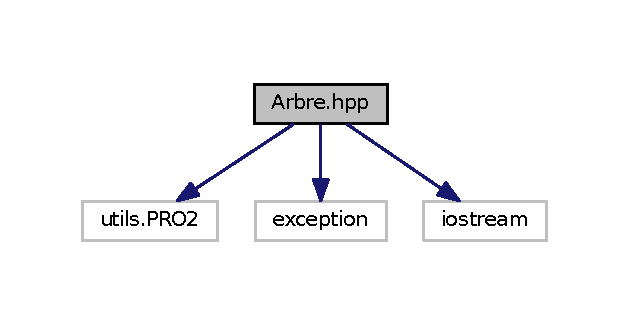
\includegraphics[width=302pt]{_arbre_8hpp__incl}
\end{center}
\end{figure}
\subsection*{Clases}
\begin{DoxyCompactItemize}
\item 
class \hyperlink{class_arbre}{Arbre$<$ T $>$}
\item 
struct \hyperlink{struct_arbre_1_1node__arbre}{Arbre$<$ T $>$\-::node\-\_\-arbre}
\end{DoxyCompactItemize}

\hypertarget{biblioteca_8cpp}{\section{Referencia del Archivo biblioteca.\-cpp}
\label{biblioteca_8cpp}\index{biblioteca.\-cpp@{biblioteca.\-cpp}}
}
Dependencia gráfica adjunta para biblioteca.\-cpp\-:\nopagebreak
\begin{figure}[H]
\begin{center}
\leavevmode
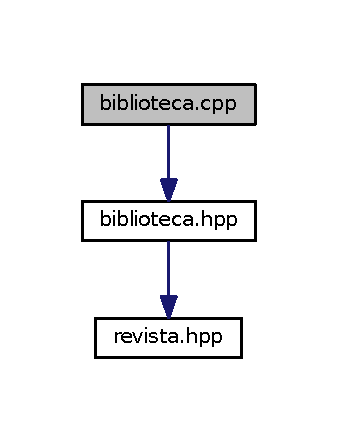
\includegraphics[width=162pt]{biblioteca_8cpp__incl}
\end{center}
\end{figure}

\hypertarget{biblioteca_8hpp}{\section{Referencia del Archivo biblioteca.\-hpp}
\label{biblioteca_8hpp}\index{biblioteca.\-hpp@{biblioteca.\-hpp}}
}
Dependencia gráfica adjunta para biblioteca.\-hpp\-:\nopagebreak
\begin{figure}[H]
\begin{center}
\leavevmode
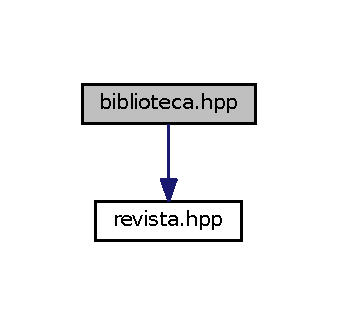
\includegraphics[width=162pt]{biblioteca_8hpp__incl}
\end{center}
\end{figure}
\subsection*{Clases}
\begin{DoxyCompactItemize}
\item 
class \hyperlink{class_biblioteca}{Biblioteca}
\end{DoxyCompactItemize}

\hypertarget{estructura_8cpp}{\section{Referencia del Archivo estructura.\-cpp}
\label{estructura_8cpp}\index{estructura.\-cpp@{estructura.\-cpp}}
}
Dependencia gráfica adjunta para estructura.\-cpp\-:\nopagebreak
\begin{figure}[H]
\begin{center}
\leavevmode
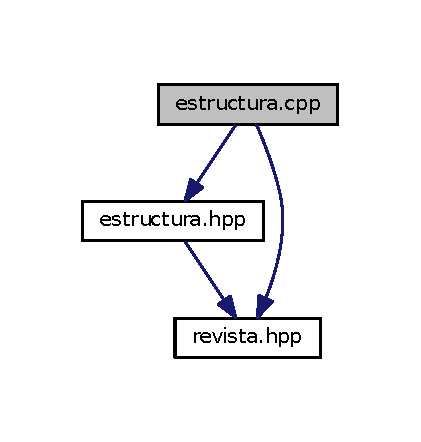
\includegraphics[width=202pt]{estructura_8cpp__incl}
\end{center}
\end{figure}

\hypertarget{estructura_8hpp}{\section{Referencia del Archivo estructura.\-hpp}
\label{estructura_8hpp}\index{estructura.\-hpp@{estructura.\-hpp}}
}
Dependencia gráfica adjunta para estructura.\-hpp\-:\nopagebreak
\begin{figure}[H]
\begin{center}
\leavevmode
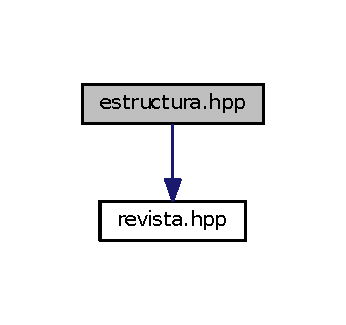
\includegraphics[width=166pt]{estructura_8hpp__incl}
\end{center}
\end{figure}
\subsection*{Clases}
\begin{DoxyCompactItemize}
\item 
class \hyperlink{class_estructura}{Estructura}
\end{DoxyCompactItemize}

\hypertarget{pro2_8cpp}{\section{Referencia del Archivo pro2.\-cpp}
\label{pro2_8cpp}\index{pro2.\-cpp@{pro2.\-cpp}}
}
Dependencia gráfica adjunta para pro2.\-cpp\-:\nopagebreak
\begin{figure}[H]
\begin{center}
\leavevmode
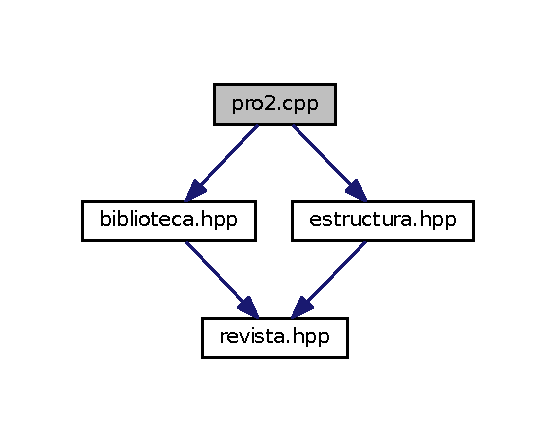
\includegraphics[width=267pt]{pro2_8cpp__incl}
\end{center}
\end{figure}
\subsection*{Funciones}
\begin{DoxyCompactItemize}
\item 
int \hyperlink{pro2_8cpp_ae66f6b31b5ad750f1fe042a706a4e3d4}{main} ()
\end{DoxyCompactItemize}


\subsection{Documentación de las funciones}
\hypertarget{pro2_8cpp_ae66f6b31b5ad750f1fe042a706a4e3d4}{\index{pro2.\-cpp@{pro2.\-cpp}!main@{main}}
\index{main@{main}!pro2.cpp@{pro2.\-cpp}}
\subsubsection[{main}]{\setlength{\rightskip}{0pt plus 5cm}int main (
\begin{DoxyParamCaption}
{}
\end{DoxyParamCaption}
)}}\label{pro2_8cpp_ae66f6b31b5ad750f1fe042a706a4e3d4}


Definición en la línea 4 del archivo pro2.\-cpp.


\begin{DoxyCode}
          \{
  \textcolor{keywordtype}{int} n = readint();
  \hyperlink{class_biblioteca}{Biblioteca} b(n);
  \hyperlink{class_estructura}{Estructura} c;
  c.\hyperlink{class_estructura_a5169bd12bdef33436dd75bdf45de18be}{llegir\_estructura}();
  \textcolor{keywordtype}{int} operacion = readint();
  \textcolor{keywordflow}{while}(operacion != -6)\{
    \textcolor{keywordflow}{if}(operacion == -1)\{    \textcolor{comment}{//ALTA REVISTA}
      \hyperlink{class_revista}{Revista} r;
      r.\hyperlink{class_revista_a61178cb7b236db9a3354d5d00df1b31b}{leer\_revista}();
      \textcolor{keywordtype}{string} area1 = c.\hyperlink{class_estructura_a756ee7e893ac64230684b5bec1497f0c}{criterio1}(r);
      \textcolor{keywordtype}{string} area2 = c.\hyperlink{class_estructura_af185388c4c717a3e77aef744b755a864}{criterio2}(r);
      r.\hyperlink{class_revista_aff45d18000f503ccaaba3fe8f956661c}{modificar\_AreasTematicas}(area1, area2);
      b.anadir\_revista(r);
    \}
    \textcolor{keywordflow}{else} \textcolor{keywordflow}{if}(operacion == -2)\{
      \textcolor{keywordtype}{string} r1 = readstring();
      b.eliminar\_revista(r1);
    \}
    \textcolor{keywordflow}{else} \textcolor{keywordflow}{if}(operacion == -3)\{   \textcolor{comment}{//FUSIONAR REVISTAS}
      \textcolor{keywordtype}{string} r1, r2;
      r1 = readstring();
      r2 =  readstring();
      \textcolor{keywordtype}{bool} b1;
      list<Revista>::iterator it;
      b.fusionar\_revistas(r1, r2, it, b1);
      \textcolor{keywordflow}{if}(b1)\{
        \hyperlink{class_revista}{Revista} r = (*it);
        \textcolor{keywordtype}{string} area1 = c.\hyperlink{class_estructura_a756ee7e893ac64230684b5bec1497f0c}{criterio1}(r);
        \textcolor{keywordtype}{string} area2 = c.\hyperlink{class_estructura_af185388c4c717a3e77aef744b755a864}{criterio2}(r);
        r.\hyperlink{class_revista_aff45d18000f503ccaaba3fe8f956661c}{modificar\_AreasTematicas}(area1, area2);
        \textcolor{keywordtype}{int} calidad  = (*it).consultar\_calidad();
        b.reordenar\_areas(r, calidad, r1, it);
      \}
    \}
    \textcolor{keywordflow}{else} \textcolor{keywordflow}{if} (operacion == -4)\{
      \textcolor{keywordtype}{int} calidad = readint();
      \textcolor{keywordtype}{int} criterio = readint();
      cout << \textcolor{stringliteral}{"Revistas de calidad "} << calidad << \textcolor{stringliteral}{" por criterio "} << criterio
       << endl;
      \textcolor{keywordflow}{if}(criterio == 1) b.listar\_criterio1(calidad);
      \textcolor{keywordflow}{else} b.listar\_criterio2(calidad);
      cout << endl;
    \}
    \textcolor{keywordflow}{else} \textcolor{keywordflow}{if} (operacion == -5)\{    \textcolor{comment}{//CONSULTA DE REVISTAS POR TÍTULO}
      \textcolor{keywordtype}{string} r1 = readstring();
      cout << \textcolor{stringliteral}{"Consulta de revista por titulo"}<< endl;
      list<Revista>::iterator it1;
      \textcolor{keywordtype}{bool} b1 = \textcolor{keyword}{false};
      b.buscar\_revista\_criterio1(r1, b1, it1);
      \textcolor{keywordflow}{if}(b1)\{
        cout << (*it1).consultar\_nombre() << endl;
        \textcolor{keywordtype}{int} tamany = (*it1).num\_pal\_clave();
        \textcolor{keywordflow}{for}(\textcolor{keywordtype}{int} i = 1; i <= tamany; ++i) \{
          cout << (*it1).consultar\_palabra\_clave(i); 
          \textcolor{keywordflow}{if}(i!= tamany) cout << \textcolor{stringliteral}{" "};
        \}
        cout << endl;
        cout << (*it1).consultar\_AreaTematica(1) << \textcolor{stringliteral}{" "} << (*it1).
      consultar\_AreaTematica(2) << endl;
        cout << (*it1).consultar\_calidad() << endl;
      \}
      \textcolor{keywordflow}{else} cout << \textcolor{stringliteral}{"La revista "} << r1 << \textcolor{stringliteral}{" no existe"}<< endl;
      cout << endl;
    \} 
    operacion = readint();
  \}
\}
\end{DoxyCode}

\hypertarget{revista_8cpp}{\section{Referencia del Archivo revista.\-cpp}
\label{revista_8cpp}\index{revista.\-cpp@{revista.\-cpp}}
}
Dependencia gráfica adjunta para revista.\-cpp\-:\nopagebreak
\begin{figure}[H]
\begin{center}
\leavevmode
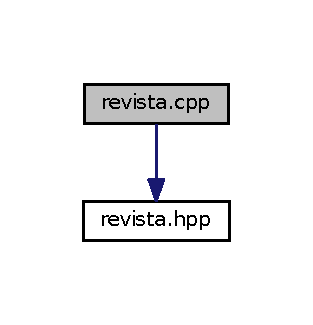
\includegraphics[width=150pt]{revista_8cpp__incl}
\end{center}
\end{figure}

\hypertarget{revista_8hpp}{\section{Referencia del Archivo revista.\-hpp}
\label{revista_8hpp}\index{revista.\-hpp@{revista.\-hpp}}
}
\subsection*{Clases}
\begin{DoxyCompactItemize}
\item 
class \hyperlink{class_revista}{Revista}
\end{DoxyCompactItemize}

\addcontentsline{toc}{part}{Índice}
\printindex
\end{document}
